\section{Deep Support Vector}\label{sec:DSV}

%This section presents the specific conditions that DSVs (Deep Support Vectors) must satisfy and discusses \jh{how to achieve that condition within gradient descent framework.}

This section presents the specific conditions that DSVs (Deep Support Vectors) must satisfy and discusses how to get an optimization loss \jh{to meet these conditions.}%the definition of an optimization loss 
% with \nj{low} computational cost that meets these conditions.


% \usepackage{algorithm}
% \usepackage{algpseudocode}


% \begin{algorithm}[tb]
%    \caption{Support Vector Refinement for Deep Learning Model}
%    \label{alg:KKT}
% \begin{algorithmic}
%    \STATE {\bfseries Input:} Pretrained model $\Phi(\cdot; \theta)$, loss function $L$, augmentation function set $A$, number of DSV candidate $N$, number of class $C$, hyperparameter $\beta$, $\gamma$, \jh{$\alpha_\lambda$, $\alpha_x$}
%    \STATE {\bfseries Ensure:} Freeze model $\Phi(\cdot; \theta)$
%    \STATE Initialize $N \times C$ number of support vector candidates
%    \FOR{$c=1$ {\bfseries to} $C$}
%    \STATE Sample $N$ number of ($x^c_i$,$\lambda^c_i$) for label $c$
%    \ENDFOR
%    \STATE Define  $X = \{ x^c_i \mid c \in [C] , i \in [N]\} $
%    \STATE Define  $\Lambda = \{ \lambda^c_i \mid c \in [C] , i \in [N]\} $
%    \REPEAT
%    \STATE $L_{\text{primal}}(X) = (\sum_{i=1}^{N}\sum_{c=1}^{C} L(\Phi(x^c_i;\theta), c))/NC$
%    \STATE$L_{\text{stat}}(X) = ||\theta + \sum_{i=1}^{N}\sum_{c=1}^{C} \lambda^c_i \nabla_\theta L(\Phi(x^c_i;\theta), c)||^2_2$
%    \STATE $L_{\text{kkt}}(X) = L_{\text{primal}}(X) + \beta \times L_{\text{stat}}(X)$
%    \STATE Sample $f_A \in A$
%    \STATE Define $X' = \{ f_A(x^c_i) \mid x^c_i \in X\} $
%    %\STATE \nj{${L_{akkt}(X)} = {L_{kkt}(X')}$ }
%    \STATE ${L_{total}(X)} = {L_{kkt}(X)} + \gamma \times {L_{kkt}(X')}$
%    \STATE Update $x_i^c \leftarrow x_i^c - \jh{\alpha_x}\nabla_{x_i^c} L_{total}(X)$, \quad  $\forall \  i \ \text{and} \ c$
%    \STATE Update $\lambda_i^c \leftarrow \lambda_i^c -\jh{\alpha_\lambda}\nabla_{\lambda_i^c} L_{total}(X)$, \quad  $\forall \  i \ \text{and} \ c$
%    \STATE Remove $x^c_i$ from $X$ if corresponding $\lambda^c_i < 0$
%    \UNTIL{$X$ converges}
%    \STATE {\bfseries Return:} Set of DSV : $X$
% \end{algorithmic}
% \end{algorithm}

% \begin{algorithm*}[h]\label{alg:KKT}
% \caption{Support Vector Refinement for Deep Learning Model}
% \begin{algorithmic}[1] 
% \Require Pretrained classifier $\Phi(\cdot; \theta)$, loss function $L$, augmentation function set $A$, number of DSV candidate $N$, number of class  $C$, hyperparmeter $\alpha$, $\beta$
% \Ensure Freeze classifier $\Phi(\cdot; \theta)$
% \State Initialize $N$*$C$ number of support vector candidates
% \For{i=1 to $C$}
% \State sample $N$ number of ($x^s_i$,$\lambda^s_i$) for label $y^s_i = i$
% \EndFor
% \State Define  $X^S = \{ x^s_i \mid i \in [C] , s \in [N]\} $
% \State Define  $\Lambda^S = \{ \lambda^s_i \mid i \in [C] , s \in [N]\} $
% \Repeat
%     \State $L_{\text{primal}}(X^S) = \sum_{s=1}^{N}\sum_{i=1}^{C} L(\Phi(x^s_i;\theta^*), y^s_i)$
%     \State $L_{\text{stationary}}(X^S) = ||\theta^* + \sum_{s=1}^{N}\sum_{i=1}^{C} \lambda^s_i y^s_i\nabla_\theta\Phi(x^s_i;\theta^*)||^2_2$
%     \State $L_{\text{kkt}}(X^S) = L_{\text{primal}}(X^S) + \alpha * L_{\text{stationary}}(X^S)$
%     \State Sample $f_A \in A$
%     \State Define $AX^S = \{ f_A(x^s_i) \mid x^s_i \in X^S\} $
%     \State ${L_{akkt}(X^S)} = {L_{kkt}(AX^S)}$ 
%     \State ${L_{total}(X^S)} = {L_{kkt}(X^S)} + \beta * {L_{akkt}(X^S)}$
%     \State Update $X^S \longleftarrow X^S + \nabla_{X^S} L_{total}(X^S) $
%     \State Update $\Lambda^S \longleftarrow \Lambda^S + \nabla_{\Lambda^S} L_{total}(X^S) $
%     \State Remove $x^s_i$s for corresponding $\lambda^s_i < 0$
% \Until{$X^S$ converges}
% \State \Return Set of DSV : $X^S$
% \end{algorithmic}
% \end{algorithm*}


% \begin{algorithm*}[h]\label{alg:KKT}
% \caption{Support Vector Refinement for Deep Learning Model}
% \begin{lstlisting}[language=Python, frame=single, numbers=left, mathescape=true]
% # Required objects: Trained model $f$, loss function $L$, augmentation functor $A$, 
% # number of DSV candidate $N$, number of class  $C$ (output dimension of trained model)

% # Initialize $Nㅎ_C$ number of support vector candidates
% for i in range(C):
%     # sample N number of $x_s$ which has label $y_s$ = i

% while not converged:
%     # Compute KKT condition
%     $L_{\hh{primal}}($x_s$)$ = L(f($x_s$), $y_s$)
%     $L_{\hh{stat}}($x_s$)$ =  (theta_star - $\Sigma$(lambda_i * grad(L_primal, $x_s[i]$)))
%     $L_{\hh{kkt}}($x_s$)$ = $L_{\hh{primal}}($x_s$)$ + $\alpha$ * $L_{\hh{stat}}($x_s$)$

%     $ax_s$ = A($x_s$)
%     # calculate $L_kkt$ using $ax_s$ and name it $L_akkt$
%     $\hh{L_{akkt}(x_s)}$ = $\hh{L_{kkt}(ax_s)}$
%     Loss = $L_{\hh{kkt}}(x_s)$ + beta * $L_{\hh{akkt}}($x_s$)$
%     update x_s, lambda using Loss. Discard x_s[i] if lambda[i] < 0
%     update_support_vectors(...)
% \end{lstlisting}
% \end{algorithm*}

\subsection{DeepKKT}
\label{sec:deepkkt}

\paragraph{%Viewpoint of gradient descent with hinge loss}
SVM's Relationship with Hinge loss}

%We start our discussion by applying the gradient descent module to SVM directly. When we perform gradient descent with the hinge loss in linear model $w$, the optimized $\tilde{w}^*$ satisfies KKT condition without complementary slackness.

%Suppose we initialize weight $\tilde{w}$ with 0, and optimize it with gradient descent with learning rate $\alpha$
%
% \begin{equation}
% \text{Hinge Loss:} \quad L = \frac{1}{N} \sum_{i=1}^N \max(0, 1 - y_i(\tilde{w}^T \tilde{x}_i))
% \end{equation}
%
% \begin{equation}
% \frac{\partial L}{\partial w} = \frac{1}{N} \sum_{i=1}^N \left\{ \begin{array}{ll} 0, & \text{if } y_i(w^T x_i) \geq 1 \\ -y_i x_i, & \text{otherwise} \end{array} \right.
% \end{equation} \label{eq:hingegrad}
%
%
% As in eq~\ref{eq:hingegrad}, we can notice that gradient does not flow for $x_i$ if and only if the model satisfies primary condition. So define $\beta_i \in \mathbf{N}$ which is a number of effectve gradient numbers Suppose we performed gradient descent $T$ times, then the gradient corresponds $x_i$ actually flows if and only if the model does not satisfied primal condition.  Suppose we conducted gradient descent $T$ times, and we achieved 100\% for training set \footnote{Following condition is natural as general deep learning exploits overparameterized, settting. \ie Accuracy amoing training sets are 100\%}. Then the converged weight $w^\star$ becomes
% As in eq~\ref{eq:hingegrad}, we can notice that gradient does not flow for $x_i$ if and only if the model satisfies primary condition. So define $\beta_i \in \mathbf{N}$ which is a number of effectve gradient numbers Suppose we performed gradient descent $T$ times, then the gradient corresponds $x_i$ actually flows if and only if the model does not satisfied primal condition.  Suppose we conducted gradient descent $T$ times, and we achieved 100\% for training set \footnote{Following condition is natural as general deep learning exploits overparameterized, settting. \ie Accuracy amoing training sets are 100\%}. Then the converged weight $w^\star$ becomes
%

We start our discussion by focusing on the \textit{hinge loss,} a continuous surrogate loss for the primal feasibility, and its gradient:
\begin{equation}
\begin{split}
&\text{Hinge Loss:} \ L_h(x_i, y_i; \tilde{w}) = \frac{1}{n} \sum_{i=1}^n \max(0, 1 - y_i(\tilde{w}^T \tilde{x}_i)), \\
%\end{equation*}
%and the gradient of which becomes
%\begin{equation}
\label{eq:hingegrad}
& \quad\nabla_{\tilde{w}}  L_h = \frac{1}{n} \sum_{i=1}^n \begin{cases} 0, & \text{if } y_i(\tilde{w}^T \tilde{x}_i) \ge 1 \\ -y_i \tilde{x}_i, & \text{otherwise.} \end{cases}
\end{split}
\end{equation}
%
With Eq.~(\ref{eq:hingegrad}), the stationarity condition \nj{of SVM} becomes 
\begin{equation}\label{eq:hingesvm}
w^* := -\sum_{i=1}^{n} \alpha_i \nabla_w L_{\jh{h}}(x_i, y_i;w^*), \quad \text{s.t.} \  \alpha_i \ge 0.
\end{equation}


\paragraph{Generalization of conventional KKT conditions}

In this paper, we \nj{extend} the KKT conditions %presented in Eq.~(\ref{eq:KKT}) 
to deep learning. In doing so, the two main hurdles of a deep network different from a linear binary SVM are 1) the nonlinearity of $\Phi(x_i;\theta)$ taking the role of $\tilde{w}^T \tilde{x}_i$ and 2) multi-class nature of a deep learning model. 


Considering \nj{that} the role of the \nj{primal feasibility} condition is to correctly classify $x_i$ into $y_i$, we can enforce the score $\Phi_{y_i}(x_i;\theta)$ for the correct class $y_i$ to take the maximum value among all the logits with some margin $\epsilon$, \ie 
\begin{equation}
    \Phi_{y_i}(x_i; \theta^*) - \max_{c\neq y_i, c\in [C]} \Phi_{c}(x_i; \theta^*) \ge \epsilon, 
    \label{eq:primal}
\end{equation} 
% Because this condition is discontinuous, we can relax it with a surrogate function $-L(\Phi(x_i; \theta^*), y_i)$, which is the negative loss function to maximize. Note that if we take the cross-entropy loss for $L$, it becomes 
\jh{We can relax \nj{this discontinuity with a continuous surrogate function} $-L(\Phi(x_i; \theta^*), y_i)$, which is the negative loss function to maximize. Note that if we take the cross-entropy loss for $L$, it becomes}
\begin{equation}
-L_{ce} = \Phi_{y_i}(x_i; \theta^*) - \log \sum_{c=1}^C \exp (\Phi_{c}(x_i; \theta^*)),
\label{eq:primal_ce}
\end{equation}
which takes a similar form as Eq.~(\ref{eq:primal}) and the negative loss can be maximized to meet the condition.


\begin{table}[t]
  \centering
  \resizebox{0.5\linewidth}{!}{
    \begin{tabular}{l|l|rr}
      \hline
      img/cls & ratio (\%) & \multicolumn{1}{l}{Random} & \multicolumn{1}{l}{selected DSVs } \\ \hline
      50      & 1          & 46.16 $\pm$ 1.93           & 48.91 $\pm$ 0.90               \\
      10      & 0.2        & 30.08 $\pm$ 1.96           & 33.69 $\pm$ 2.05               \\
      1       & 0.02       & 14.26 $\pm$ 0.99           & 16.83 $\pm$ 0.29               \\ \hline
    \end{tabular}
  }
  \vspace{5mm}
  \caption{\jh{In coreset selection benchmarks \nj{using the CIFAR-10 dataset, the DeepKKT condition is used as the selection criterion. Images with the highest $\lambda$ for each class were chosen to train a network. }}}
  \label{table:coreset}
\end{table}


Now that we found the analogy between $y_i\tilde{w}^T\tilde{x}_i$ and $-L(\Phi(x_i; \theta^*), y_i)$, $y_i \tilde{x}_i (=\nabla_{\tilde{w}} (y_i\tilde{w}^T\tilde{x}_i))$ corresponds to $-\nabla_{\theta^*} L(\Phi(x_i; \theta^*), y_i)$. Thus, the stationary condition $\tilde{w} = \sum_{i=1}^n \alpha_i y_i \tilde{x}_i$ in SVMs can be translated into that of deep networks such that
\begin{equation}
\theta^* = - \sum_{i=1}^n \lambda_i \nabla_{\theta^*} L(\Phi(x_i; \theta^*), y_i).
\end{equation}
%
This condition is a generalized formulation of Eq.~(\ref{eq:hingesvm}), where we substitute the linear model $\tilde{w}^T \tilde{x}$ with a nonlinear model $\Phi(x; \theta)$, and the binary classification hinge loss $L_h$ with multi-class classification loss $L$. \jh{Furthermore, the stationarity condition reflects the dynamics of overparameterized deep learning models. We provide an analogy \nj{with respect to \cite{svm:theory}} in Appendix~\ref{sec:overparam}.}


However, these conditions are not enough for deep learning. As mentioned before, \jh{we are interested in dealing with high dimensional manifolds.} Compared to the problems dealt with in the classical SVMs, the input dimensions of deep learning problems are typically much higher. %  increased considerably.} % For classical machine learning, it deals with low dimension. However, for deep learning, it deals with high dimension. 
In this case, the data are likely to lie along a low-dimensional latent manifold $\mathcal{M}$ inside the high-dimensional space. %$\mathcal{D}$ lies in \nj{an} ambient space. \ie it forms a manifold. 
To \nj{make} a generated sample be a plausible DSV,  it not only should satisfy the generalized KKT condition but also should lie in an appropriate data manifold, \ie $x \in \mathcal{M}$.


Finally, we can rewrite the new \textbf{DeepKKT condition} as follows:
%
\begin{equation} \label{eq:DeepKKT}
\begin{aligned}
&\text{Primal feasibility:} && 
\forall\, i \in \mathcal{I}, \quad \argmax_c\; \Phi_c (x_i; \theta^*) = y_i \\
%\jh{\forall argmax \Phi(X_i; \theta^*) = y_i}, \\%  \nj{\Phi_{y_i}(x_i; \theta^*) \geq 1}\\ 
&\text{Dual feasibility:} && \forall\, i \in \mathcal{I}, \quad \lambda_i \geq 0, \\
% &\text{CS condition:} 
%&\text{slackness:} 
% && \forall\, i \in \mathcal{I}, \quad % \in [n],
% \ \nj{\lambda_i (y_i \Phi(x_i; \theta^*) - 1) = 0}, \\
&\text{Stationarity:} && \theta^* = -\sum_{i=1}^n \lambda_i \nabla_{\theta} \mathcal{L}(\Phi(x_i; \theta^*), y_i), \\
&\text{Manifold:} && \forall\, i \in \mathcal{I}, \quad x_i \in \mathcal{M}. 
\end{aligned}
\end{equation}
%
% \jh{In overparameterized deep learning models, a condition of stationarity naturally emerges, as illustrated in Fig.~\ref{fig:intuitive_stat}. This phenomenon is particularly evident in scenarios with separable data, where the model reaches 100\% training accuracy. Despite achieving this level of accuracy, the loss does not drop to zero, mainly due to the logistic tail present in commonly used loss functions like cross-entropy loss. Consequently, even after attaining perfect accuracy on the training set, the model continues to overfit. This overfitting leads to a convergence of the gradient direction. In an infinite training epoch scenario, this results in the normalized weight vector \(\hat{w} = \frac{w}{\lvert w \rvert}\) aligning with the direction of the negative, converged gradient. This aligns with the concept of stationarity in the dynamics of overparameterized models. This analogy illustrates that even with diminishing loss, the model can still converge towards a specific gradient direction, akin to the infinite series \(\sum_{i=1}^\infty \frac{1}{n} = \infty\), which suggests that small contributions can accumulate to significant effects. }



%
% \jh{Also, the modified stationarity reflects modern dynamics of overparameterized deep learning. Fig.~\ref{fig:intuitive_stat} explains this dynamics. For separable data \ie when model achieves 100\% accuracy on training set, with gradient descent learning, the model follows negative direction of gradients along the optimiziation direction even if the model achieves 100\% on trainnig dataset, the loss is not zero as utilized loss has logistic tail (for example, cross entropy loss), so overfitting after model achieves 100\% makes the gradient direction converges and make weight follows negative direction of converged negative direction, as one normally utilized enfinite epochs, the normlized weight $\hat{w} \defeq \frac{w}{|w|}$ becomes the direction of negative converged gradient's direction. \footnote{물론 이때 따라서 loss의 크기도 줄어들기 때문에 해당 방향으로 수렴하지 않는다고 생각할 수 있지만, Consider $\sum_{i=1}^\infty \frac{1}{n} = \infty$를 생각해 보면, loss의 크기가 줄어든다고 할 지라도 특정 gradient 방향으로 수렴할 수 있다.}}
% % where \( \mathcal{I} \) is the index set, \( \Phi \) represents a function with parameters \( \theta^* \), and \( y_i \) is the corresponding label for each \( X_i \).
%
% \nj{위 식에서 multi-class가 사용되는데 이것을 사용할 때 $y_i$를 어떻게 설정할지에 대해서 설명할 것. 이 것 때문에 지난 번 문제가 (+냐 -냐) 생긴 게 아닐까 하는 생각이 듦. }
% \nj{아래 부분 설명은 좀 더 이해하기 쉽게 쓸 것.}
%
% \jh{TODO: 위 부분에 KKT condition에 대해ㅓ서 이야기하는 paragraph 넣기}
% \jh{1. Primal Condition 설명 \ie interpretation of Primal feasibilit, it is same as scoring function so, ...}
% \jh{2. Stationarity Condition adopting scoring perspective to the model, we paraphrase stationarity condition becomes }
% \jh{\paragraph{Primal Condition}}
% \jh{Priaml condition과 Dual conditoin은 naive하게 그대로 옮겨놓은것.}
% \jh{We neglet CS condition as we CS condition requires a measure in parameter space, which is extremely expensive.}
% \jh{또한 stationarity condition, which is our main contribution은 \ref{fig:intuitive_stat} 에서 설명하고 있는데 기존 등가성 증명 \cite{svm:theory}에서 따온 것이다.  overparameterized model 에서는 결국 gradient direction이 converge되는데, 특정 timestamp t부터 특정 방향으로만 움직인다고 가정하면, 일반적인 cross entropy와 같은 logistic loss의 경우는 loss가 절대로 0이 되지 않기 때문에 특정 timestamp T 부터는 계속해서 같은 방향으로만 parameter가 이동한다. 따라서 일반적인 infinite step에서 $w^\infty$는 converge gradient 방향으로 수렴한다.  \footnote{물론 이때 따라서 loss의 크기도 줄어들기 때문에 해당 방향으로 수렴하지 않는다고 생각할 수 있지만, Consider $\sum_{i=1}^\infty \frac{1}{n} = \infty$를 생각해 보면, loss의 크기가 줄어든다고 할 지라도 특정 gradient 방향으로 수렴할 수 있다.}}

%\vspace{-5mm}
\subsection{\jh{Deep Support Vectors, From Dust to Diamonds}}
\label{sec:DKKTcondition}

\nj{Sec.~\ref{sec:deepkkt} explored} the KKT conditions in the context of deep learning and how these conditions can be used to formulate a loss function. It is important to note that our goal is not to construct the model $\Phi$, but rather to generate \textbf{support vectors of an already-trained model $\Phi$ with its parameter $\theta^*$}.

%Our paper addresses the issue of 
\nj{To reconstruct support vectors from a trained deep learning model, sampling or synthesizing support vectors is essential}.
By replacing the optimization variable $\theta$ with $x$, we shift our focus to utilizing the DeepKKT conditions for generating or evaluating input $x$ rather than $\theta$. This adjustment necessitates a consideration of the data's inherent characteristics, specifically its multiclass nature and the tendency of the data to reside on a lower-dimensional manifold \nj{in an ambient space.} %\nj{위 문장과 아래 내용들은 4.1과 많이 겹치므로 실제 Quadratic programming으로 해결하기 보다는 typical deep learing에서의 gradient descent를 이용해서 x를 얻는다는 것만 강조할 것.}


\paragraph{Primal Feasibility}
Firstly, the primal feasibility condition \nj{in Eq.~(\ref{eq:DeepKKT}) mandates support vectors be correctly classified by the trained model $\theta^*$.}  %which is equivalent to Eq.~(\ref{eq:primal}) questions the fundamental performance of the model, \nj{\ie} the trained model $\theta^*$ must \nj{correctly discriminate} its support vectors. 
As presented in Sec.~\ref{sec:deepkkt}, instead of Eq.~(\ref{eq:primal}), we use a surrogate function %such as in Eq.~(\ref{eq:primal_ce}) 
for the loss: %first and foremost\nj{:}
%
\begin{equation}\label{eq:two_step_loss}
L_{\text{primal}} = \frac{1}{n} \sum_{i=1}^n L_i, \quad \text{where} \quad
L_i = 
\begin{cases} 
0 & \text{if } \argmax_c \Phi_c(x_i; \theta^*) = y_i, \\
L(\Phi(x_i; \theta^*), y_i) & \text{otherwise}.
\end{cases}
\end{equation}
%
% \jh{This is designed to match the primal condition by mimicking Hinge loss. When each DSV is correct, no loss is incurred. Otherwise, we compel the DSVs to predict the correct target. This also implicitly mandates complementary slackness. As $L_i$ does not increase confidence. Consequently, the final loss is computed as foㅐllows:}
This is designed to match the \nj{primal} condition by mimicking the Hinge loss. When each DSV is correctly classified, no loss is incurred. Otherwise, we adjust the DSVs to align them with the correct target, effectively optimizing the support vectors. This approach also implicitly enforces the complementary slackness condition, as $L_i$ \nj{decreases} confidence in the incorrect classification. %Consequently, the final loss, which refines the support vectors, is computed as follows:
%
%\begin{equation}\label{eq:total_loss}
%L_{\text{primal}} = \frac{1}{n} \sum_{i=1}^n L_i.
%\end{equation}
%
%
% \begin{equation}\label{eq:conditional_primal}
% L_{\text{primal}} = 
% \begin{cases} 
% 0 & \text{if } \text{argmax}(\Phi(x_i; \theta^*)) = y_i \\
% \frac{1}{n}\sum_{i=1}^n L(\Phi(x_i; \theta^*), y_i) & \text{otherwise}
% \end{cases}
% \end{equation}
%
% \begin{equation}\label{eq:primal2}
% L_{\text{primal}} = \frac{1}{n}\sum_{i=1}^n L(\Phi(x_i; \theta^*), y_i)
% \end{equation}
%
% \begin{figure}[t]  
%   \begin{minipage}[b]{.6\linewidth}
%   \centering
%     \begin{subfigure}[b]{0.48\linewidth}
%     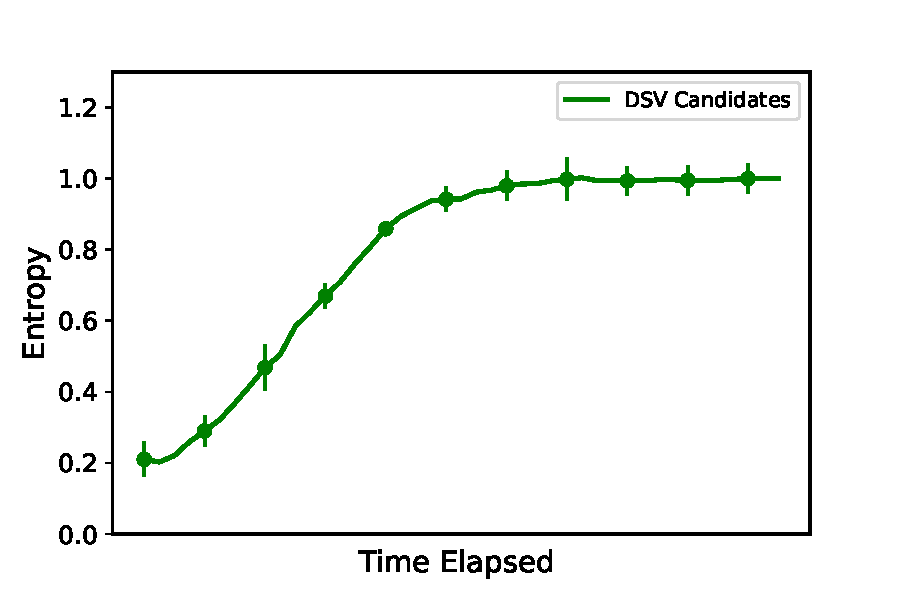
\includegraphics[width=\linewidth]{./figure/Entropy_DSV.pdf}
%     \caption{\nj{Entropy change of DSV candidates over time}}
%     \label{fig:lambda_entropy}
%   \end{subfigure}
%   \hfill
%   \begin{subfigure}[b]{0.48\linewidth}
%     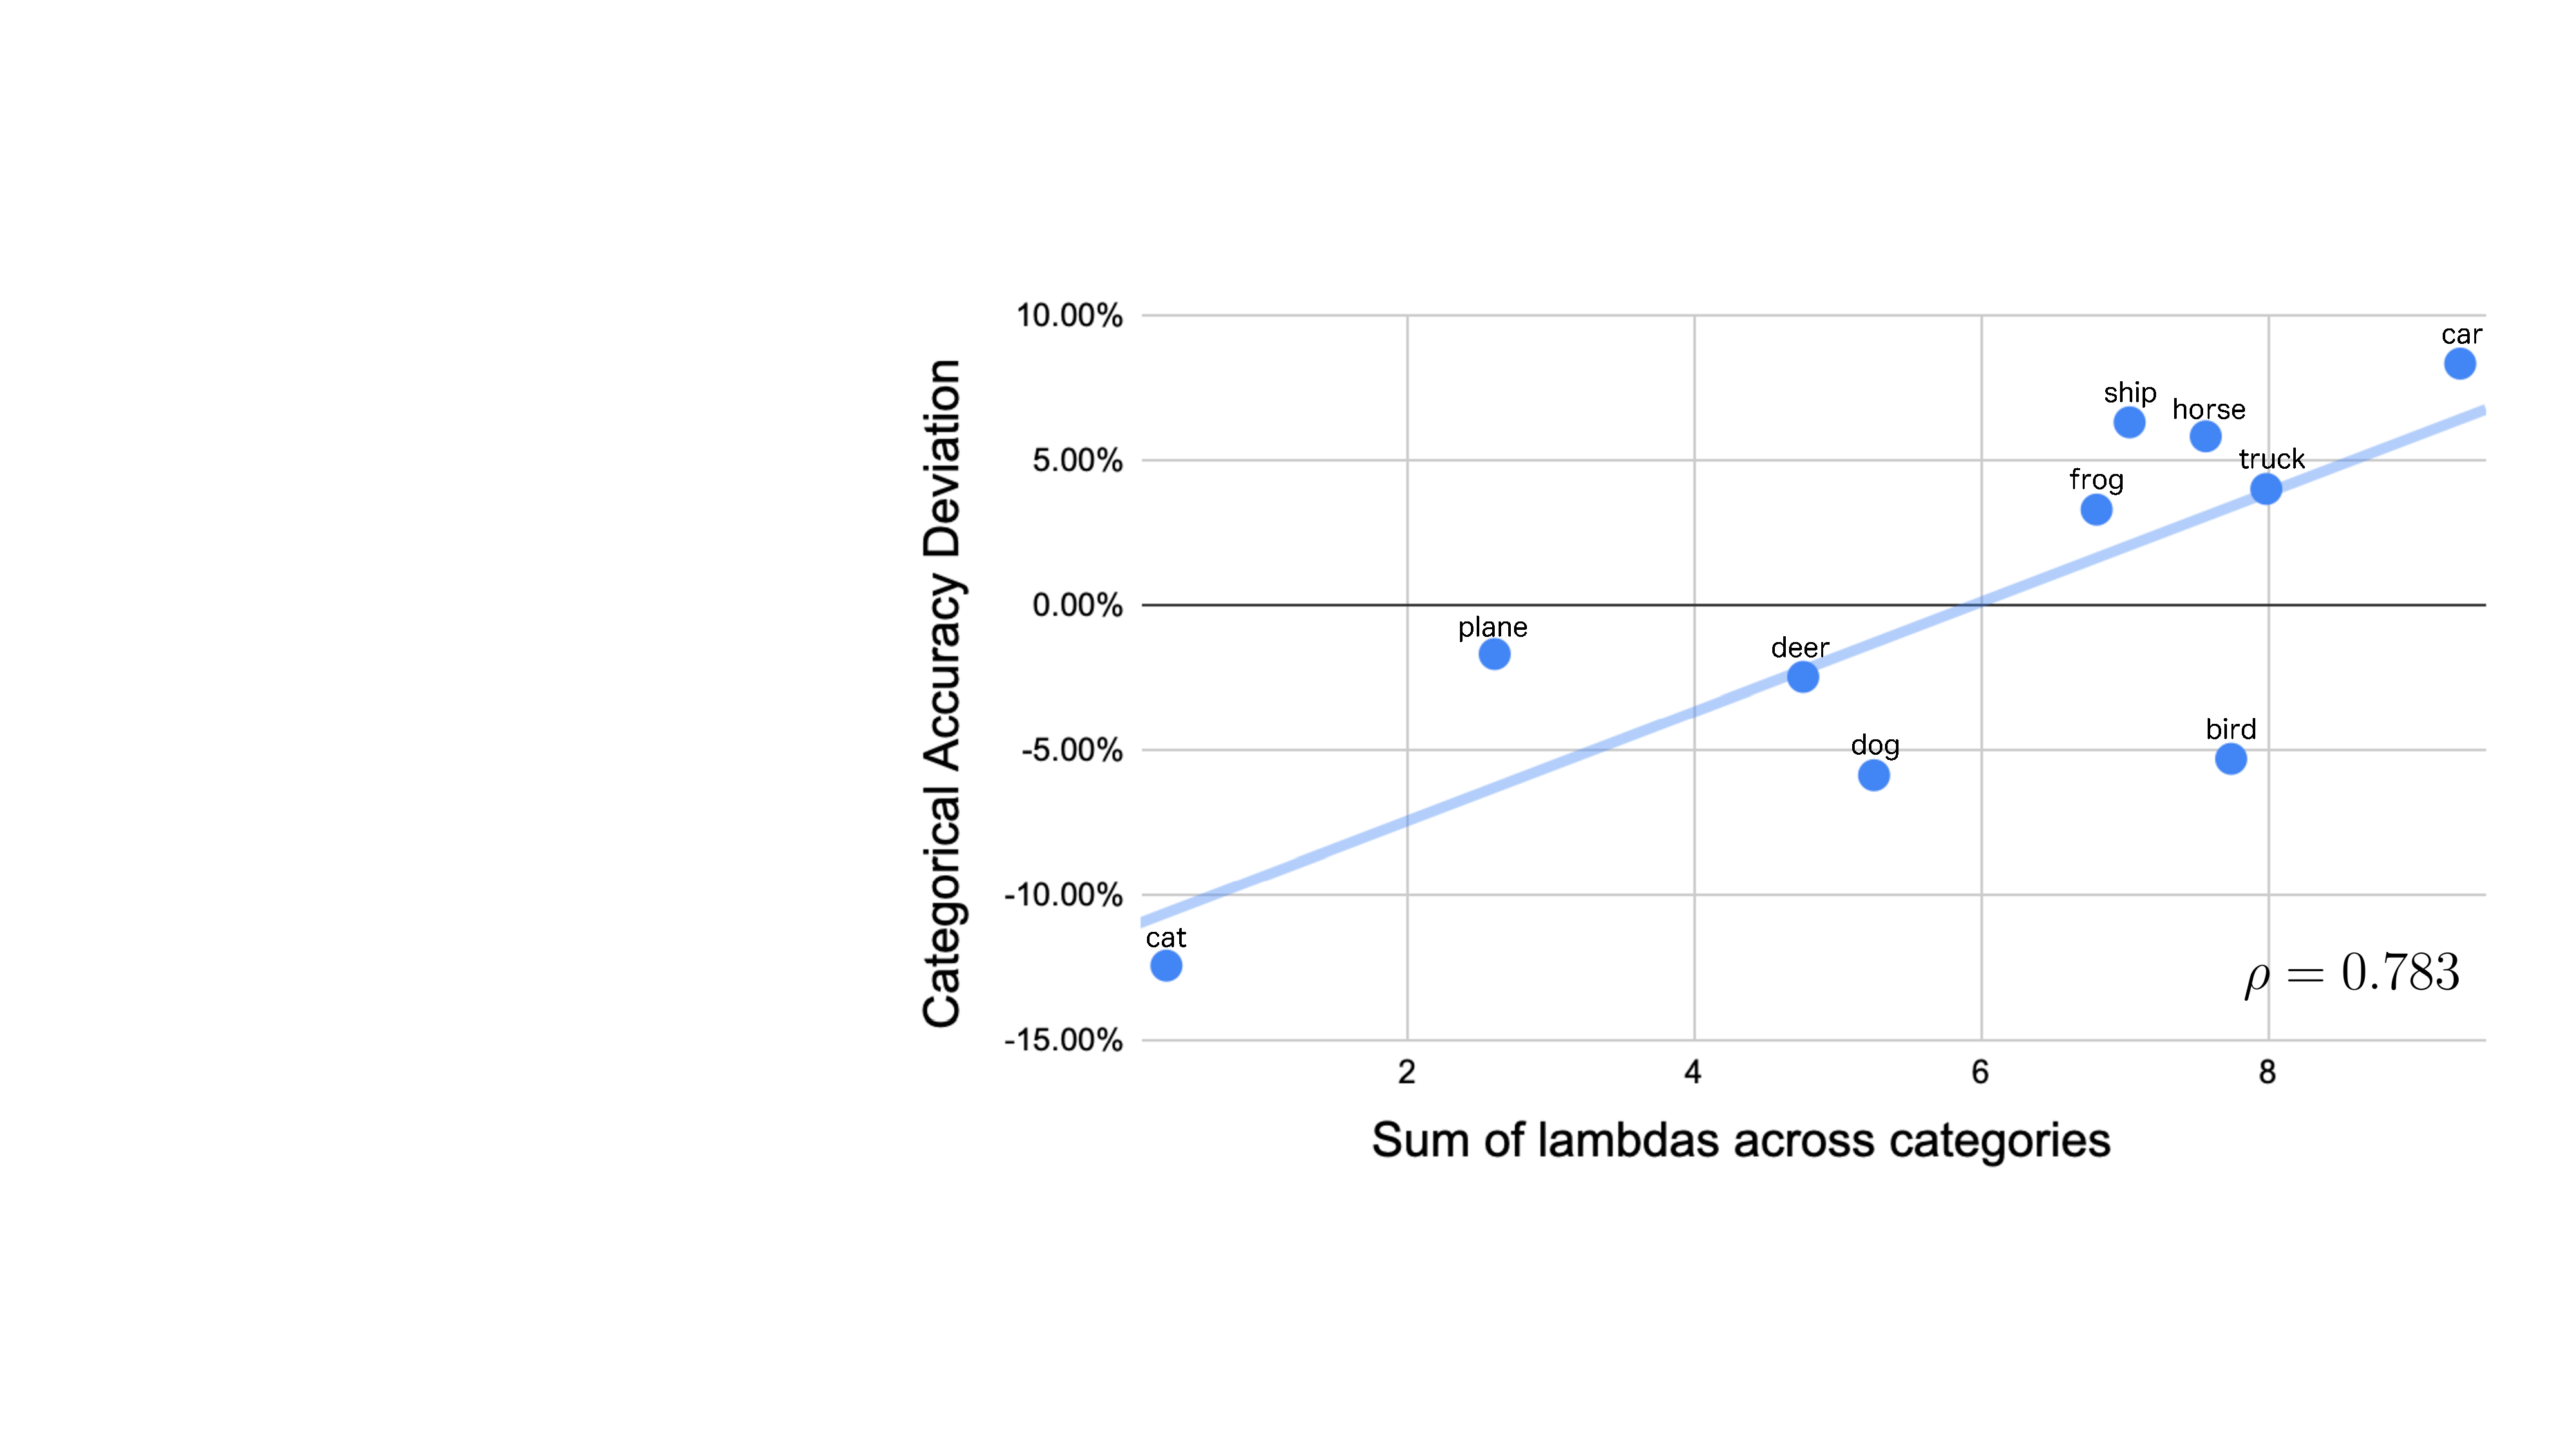
\includegraphics[width=\linewidth]{./figure/pearson.pdf}
%     \caption{Correlation between classwise mean test accuracy and \nj{the} sum of $\lambda$'s}
%     \label{fig:correlation}
%   \end{subfigure}
%   \setcounter{figure}{1}
%   \captionof{figure}{\nj{Characteristics of DSVs}%\gm{figure2여야 하는데, figure 3으로 되어있습니다}
%   }
%   \end{minipage}  
% \hfill 
% \begin{minipage}[b]{.35\linewidth}
% \vspace{-10mm}
% \centering
% \resizebox{\linewidth}{!}{
% \begin{tabular}{l|l|rr}
% \hline
% img/cls & ratio (\%) & \multicolumn{1}{l}{Random} & \multicolumn{1}{l}{selected DSVs } \\ \hline
% 50      & 1          & 46.16 $\pm$ 1.93           & 48.91 $\pm$ 0.90               \\
% 10      & 0.2        & 30.08 $\pm$ 1.96           & 33.69 $\pm$ 2.05               \\
% 1       & 0.02       & 14.26 $\pm$ 0.99           & 16.83 $\pm$ 0.29               \\ \hline
% \end{tabular}
% }
% \vspace{5mm}
% \captionof{table}{\jh{In coreset selection benchmarks \nj{using the CIFAR-10 dataset, the DeepKKT condition is used as the selection criterion. Images with the highest $\lambda$ for each class were chosen to train a network. }}}
% \label{table:coreset}
% %\end{wraptable}
% \end{minipage}
% \vspace{-5mm}
% \end{figure}

% \begin{figure}[t]
%   \centering
%   \resizebox{0.8\linewidth}{!}{%
%     \begin{minipage}{\linewidth}
%       \centering
%       \begin{subfigure}[b]{0.45\linewidth} % 첫 번째 subfigure의 폭을 45%로 설정
%         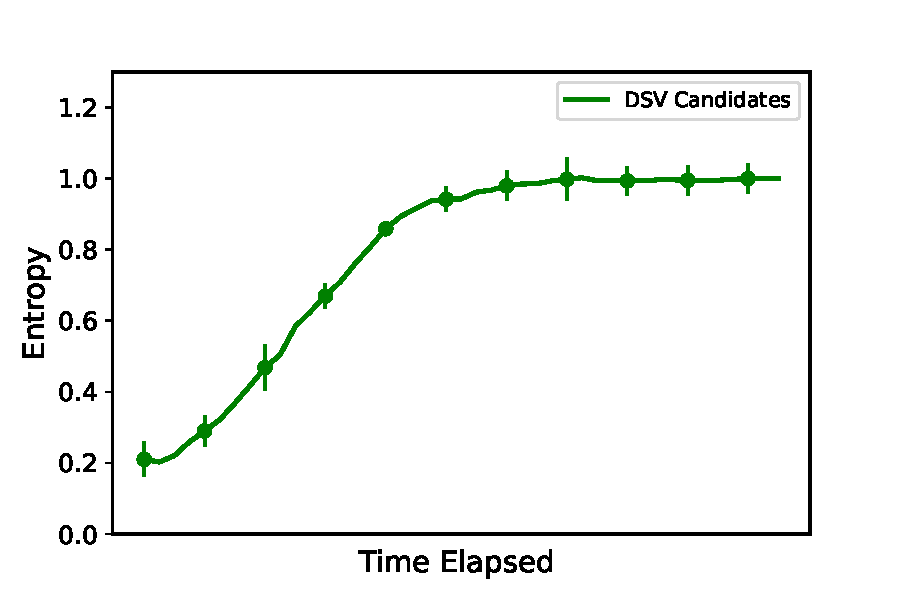
\includegraphics[width=\linewidth]{./figure/Entropy_DSV.pdf}
%         \label{fig:lambda_entropy}
%       \end{subfigure}
%       \hfill
%       \begin{subfigure}[b]{0.55\linewidth} % 두 번째 subfigure의 폭을 55%로 설정
%         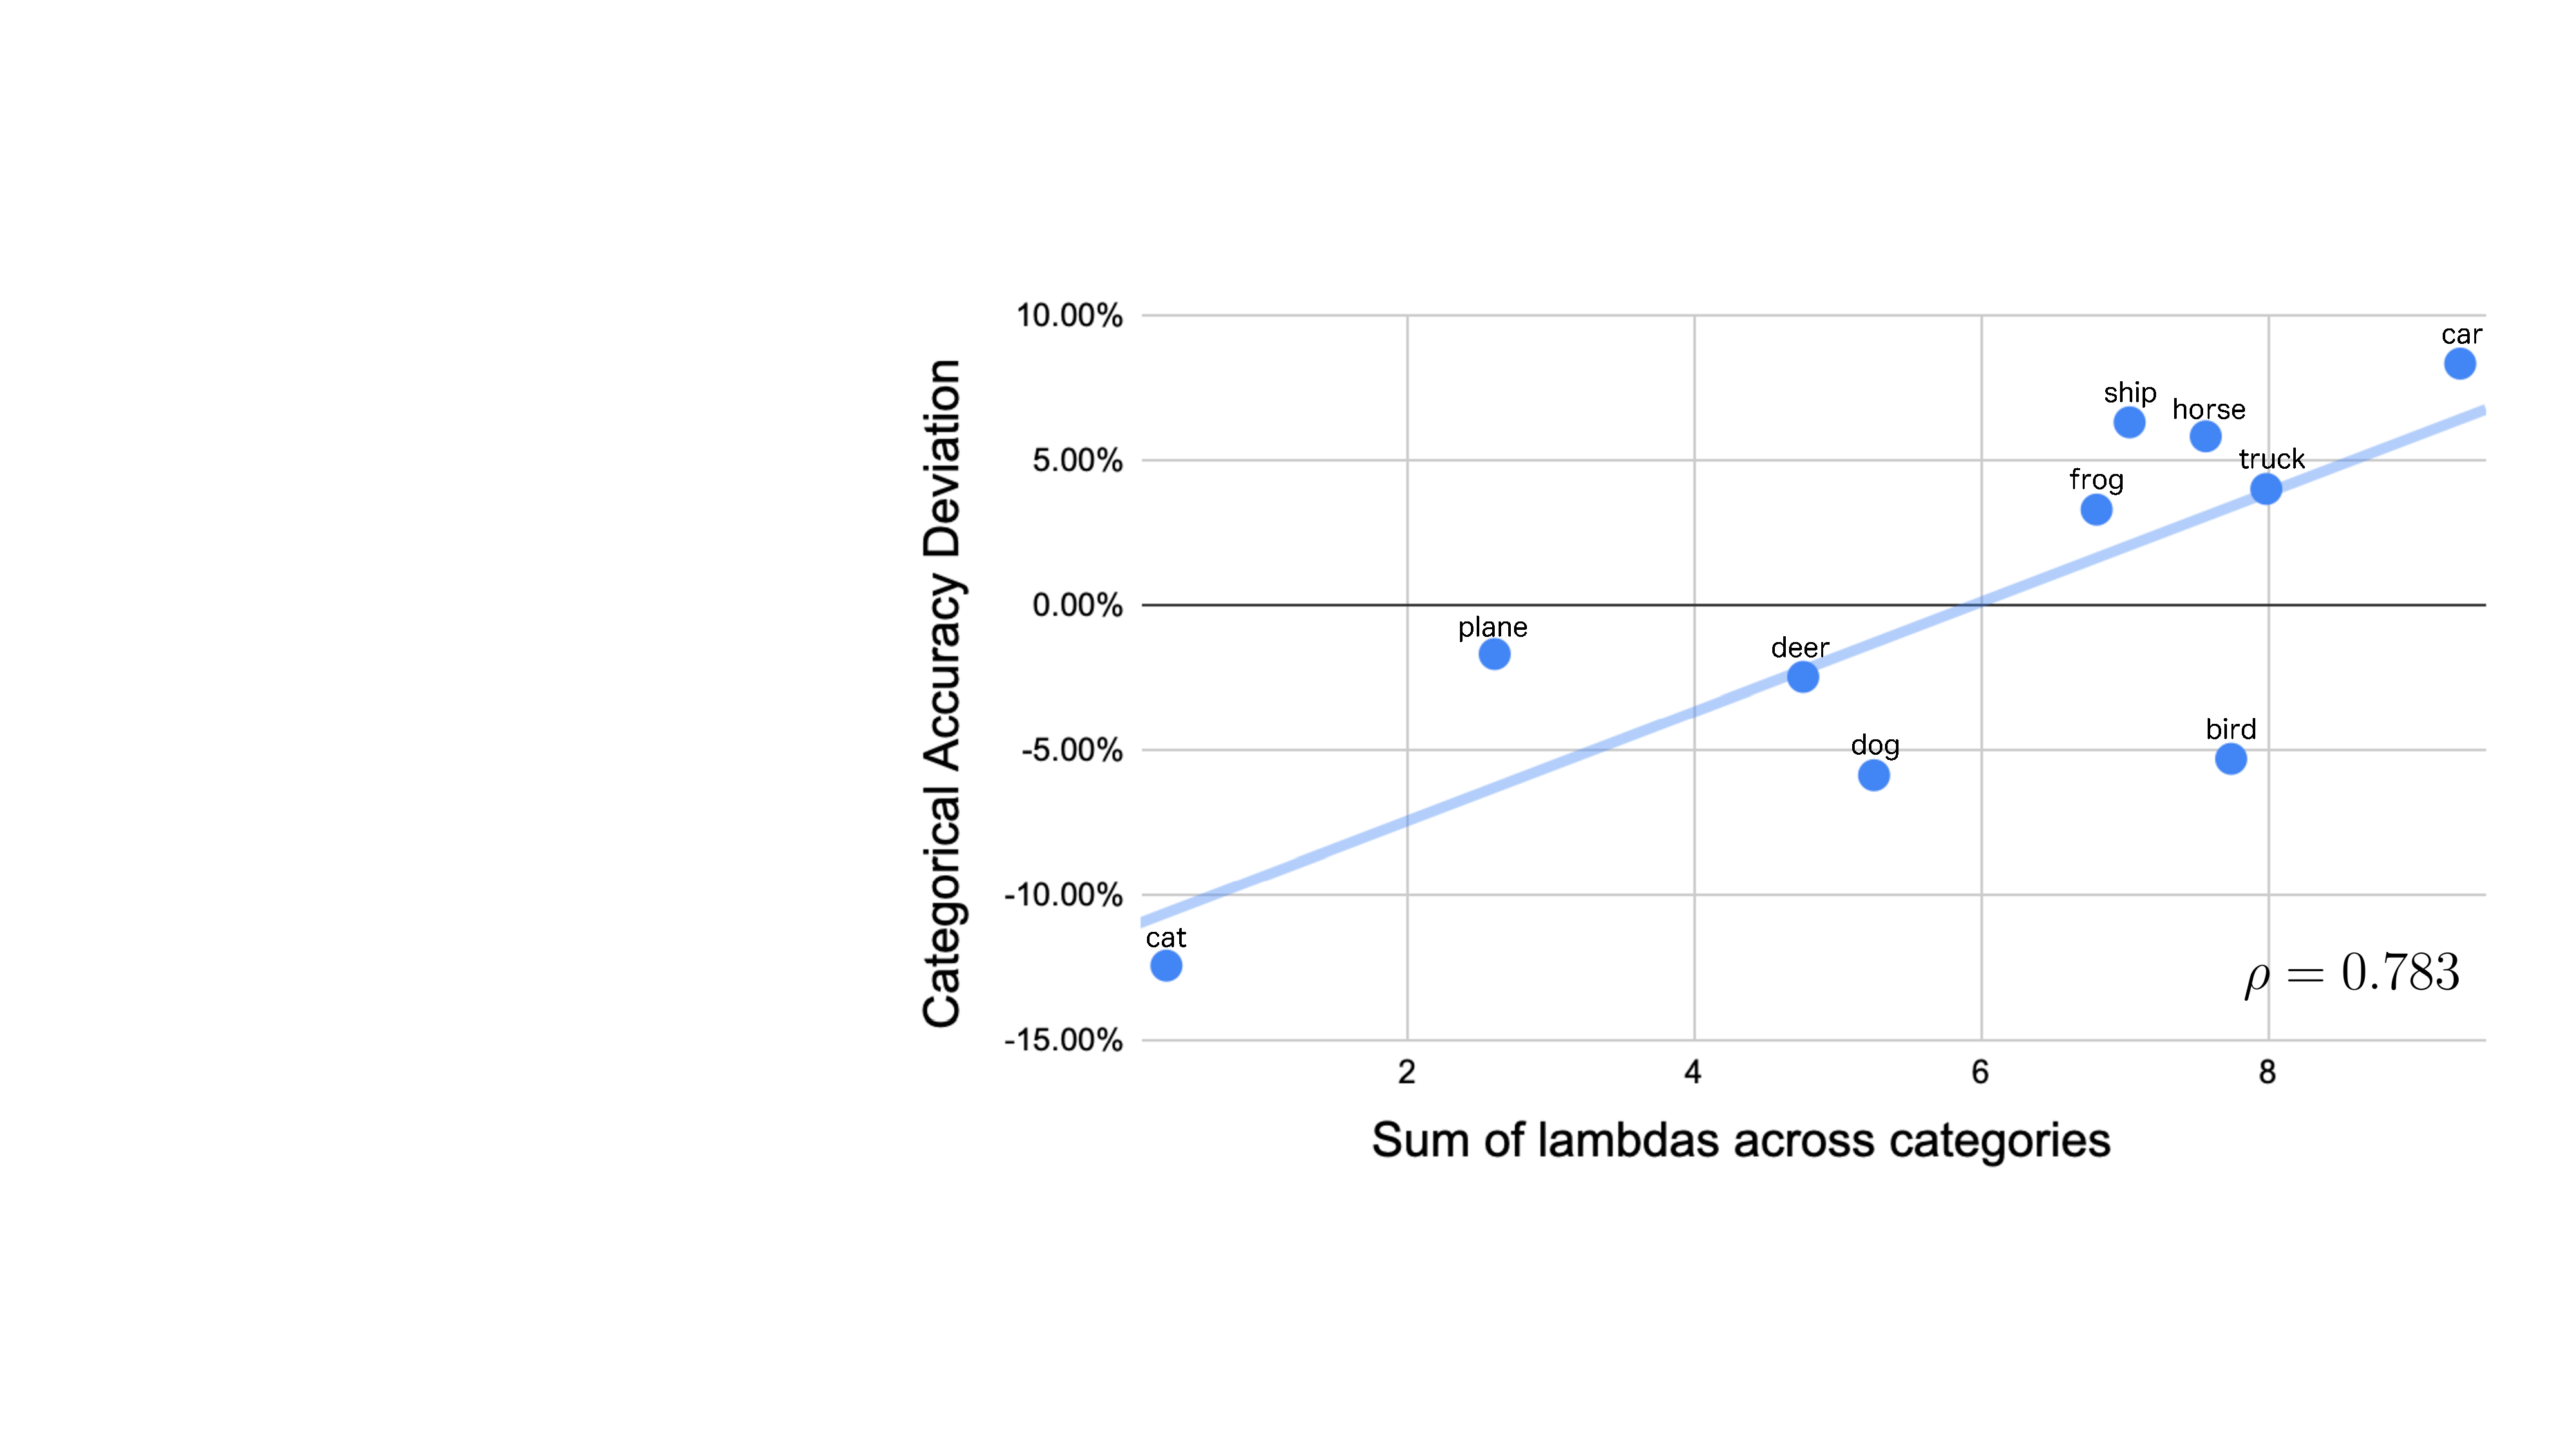
\includegraphics[width=\linewidth]{./figure/pearson.pdf}
%         % \caption{Correlation between classwise mean test accuracy and \nj{the} sum of $\lambda$'s}
%         \label{fig:correlation}
%       \end{subfigure}
%     \end{minipage}
%   }
%   % \caption{\nj{Characteristics of DSVs}}
%   \label{fig:DSV_characteristics}
% \end{figure}
  % \label{fig:DSV_characteristics}


% \begin{figure}[t]  
%   \centering
%   \begin{subfigure}[b]{0.48\linewidth}
%     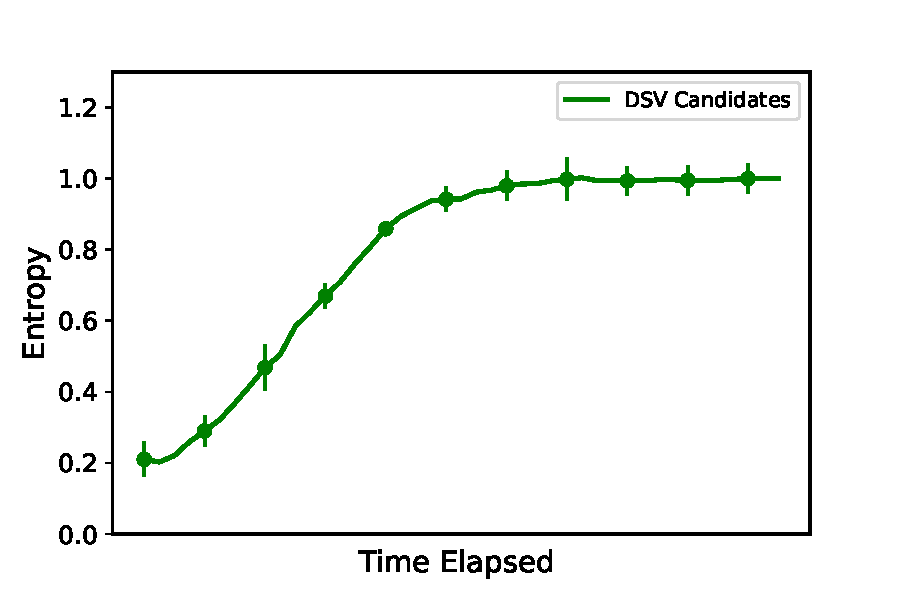
\includegraphics[width=\linewidth]{./figure/Entropy_DSV.pdf}
%     \caption{Entropy change of DSV candidates over time}
%     % \caption{}
%     \label{fig:lambda_entropy}
%   \end{subfigure}
%   \hfill
%   \begin{subfigure}[b]{0.48\linewidth}
%     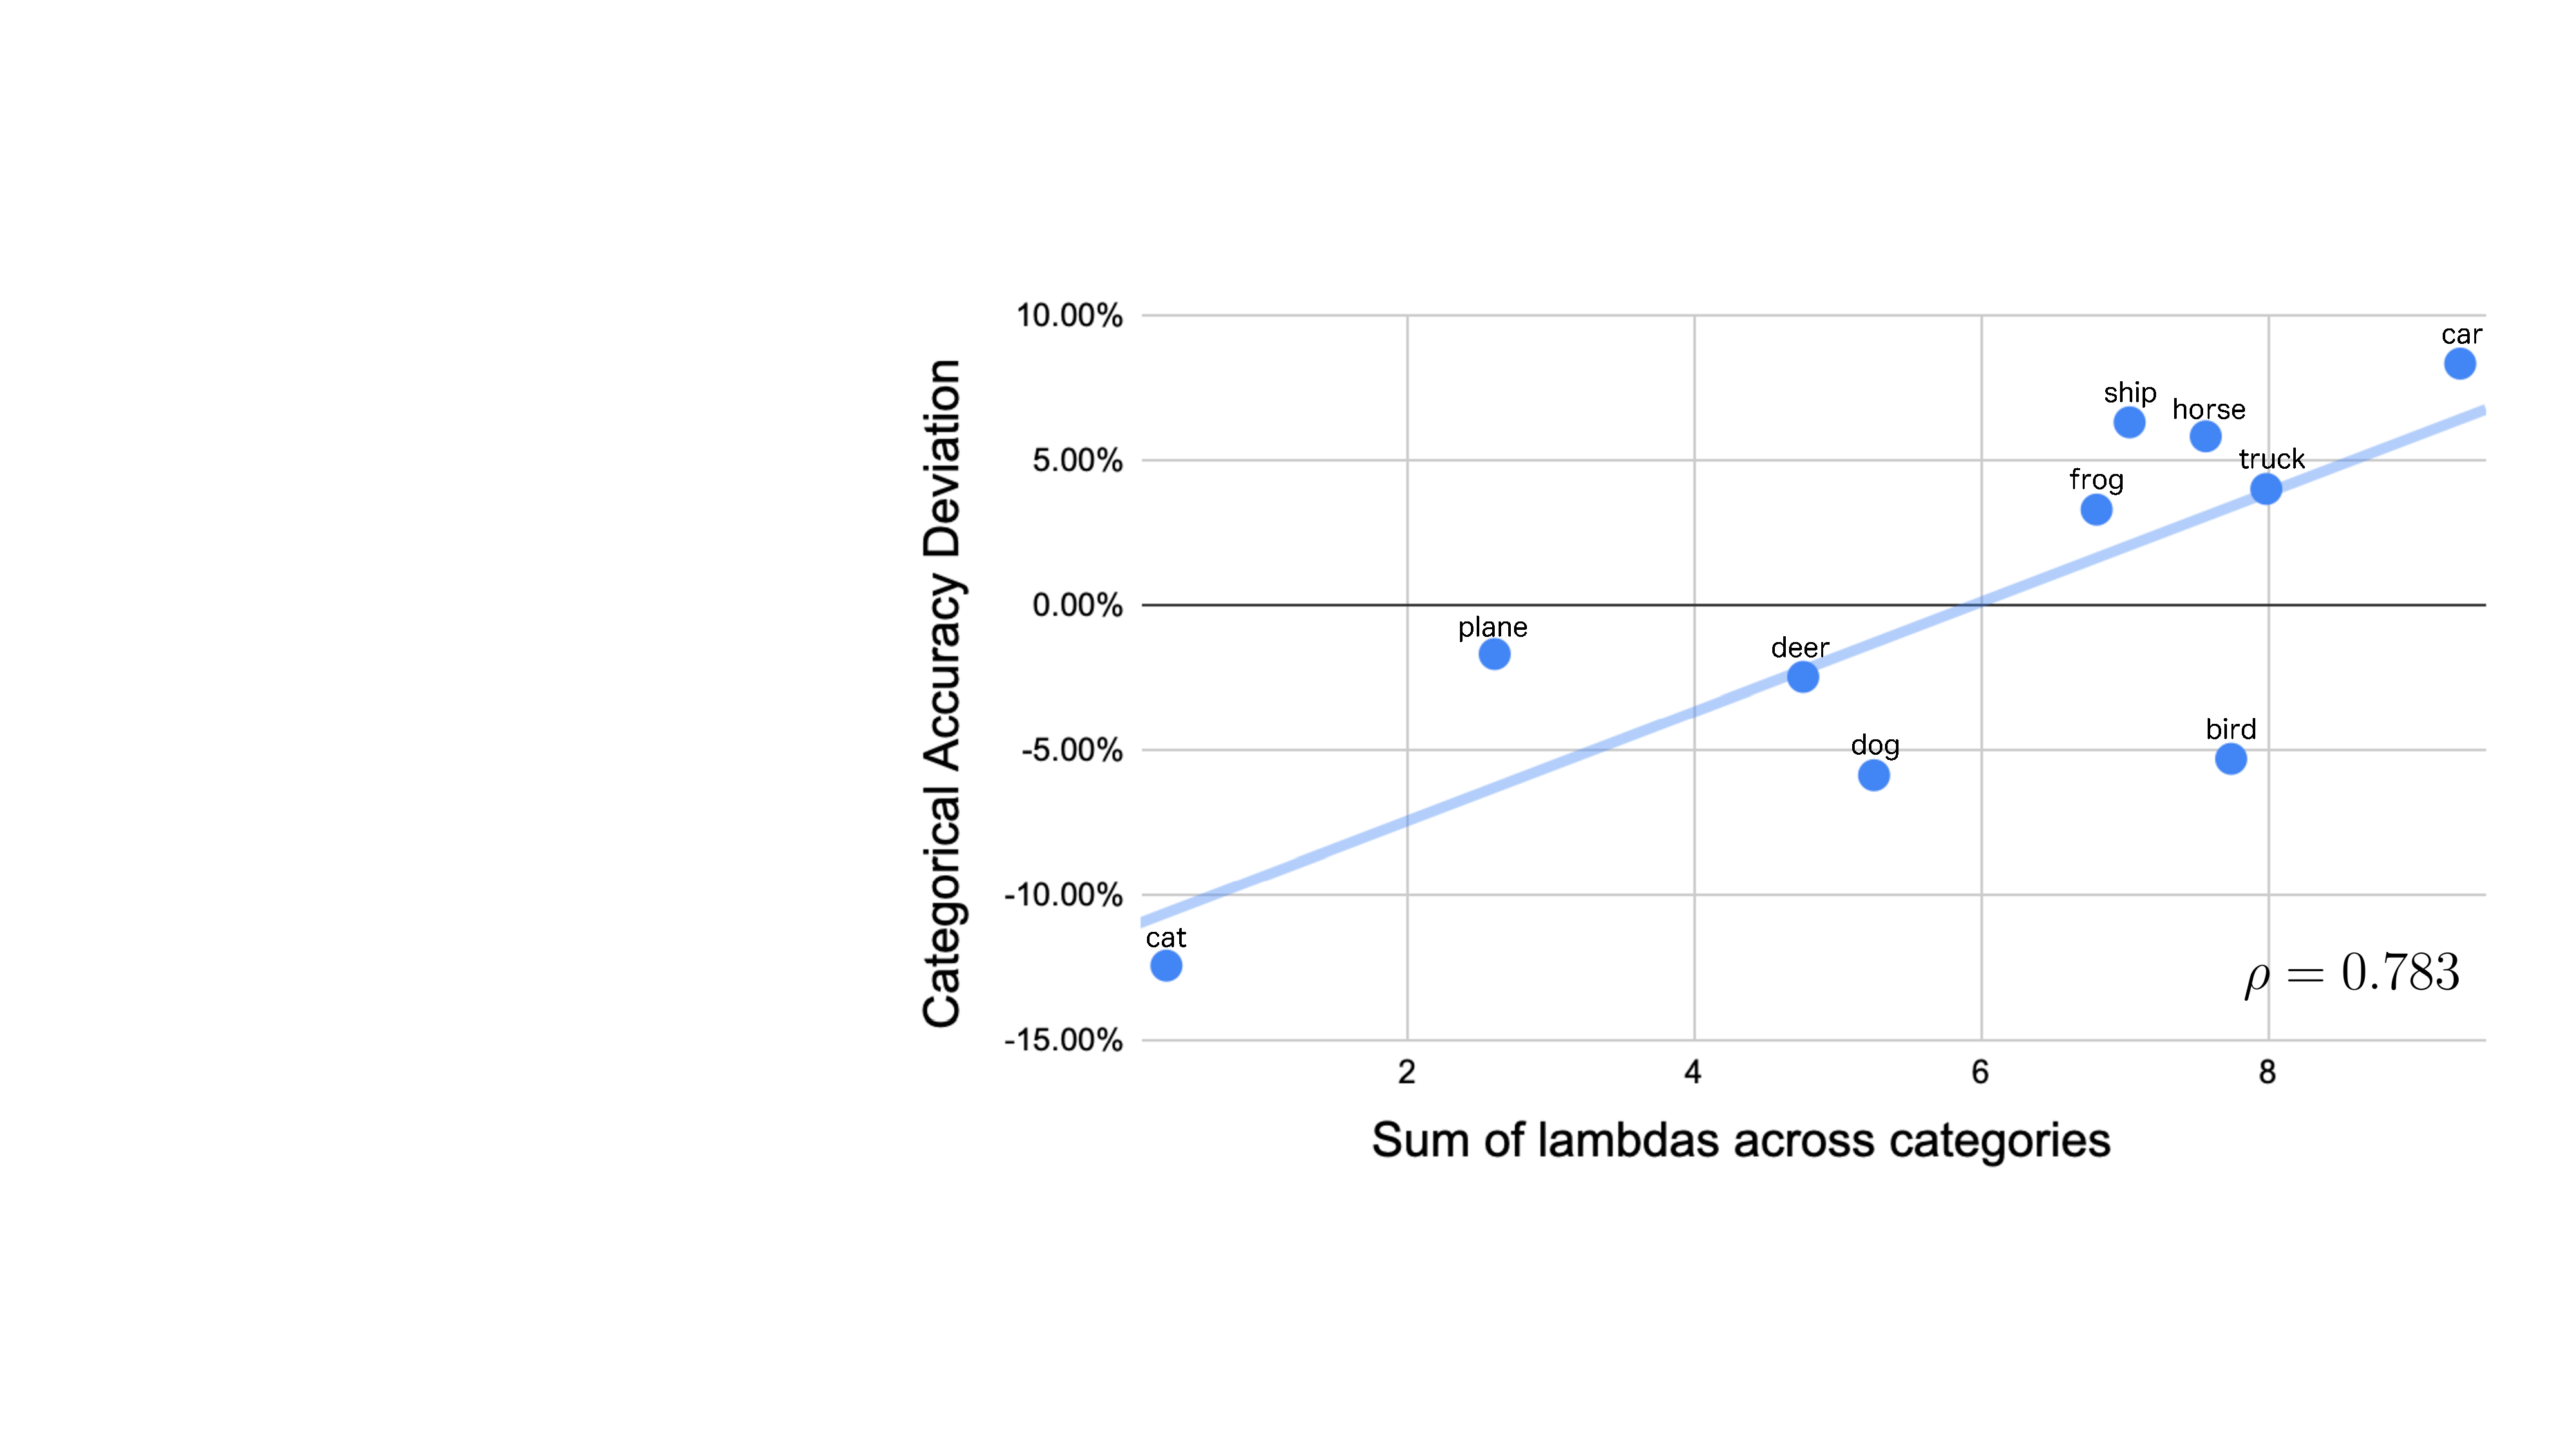
\includegraphics[width=\linewidth]{./figure/pearson.pdf}
%     % \caption*{}
%     \caption{Correlation between classwise mean test accuracy and the sum of $\lambda$'s}
%     \label{fig:correlation}
%   \end{subfigure}
%   \caption{Characteristics of DSVs}
%   \label{fig:DSV_characteristics}
% \end{figure}

% \begin{figure}[t]  
%   \centering
%   \begin{subfigure}[b]{0.48\linewidth}
%     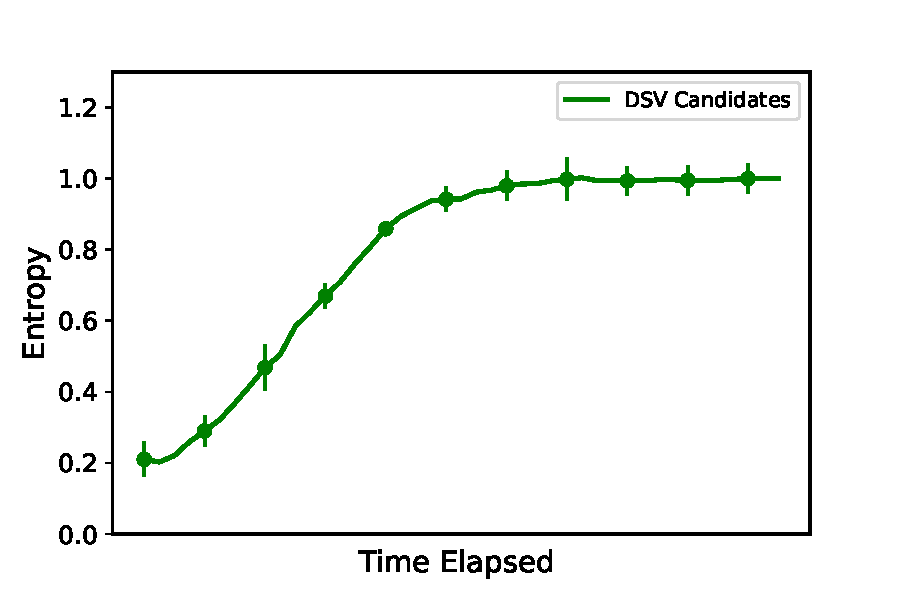
\includegraphics[width=\linewidth]{./figure/Entropy_DSV.pdf}
%     \label{fig:lambda_entropy}
%   \end{subfigure}
%   \hfill
%   \begin{subfigure}[b]{0.48\linewidth}
%     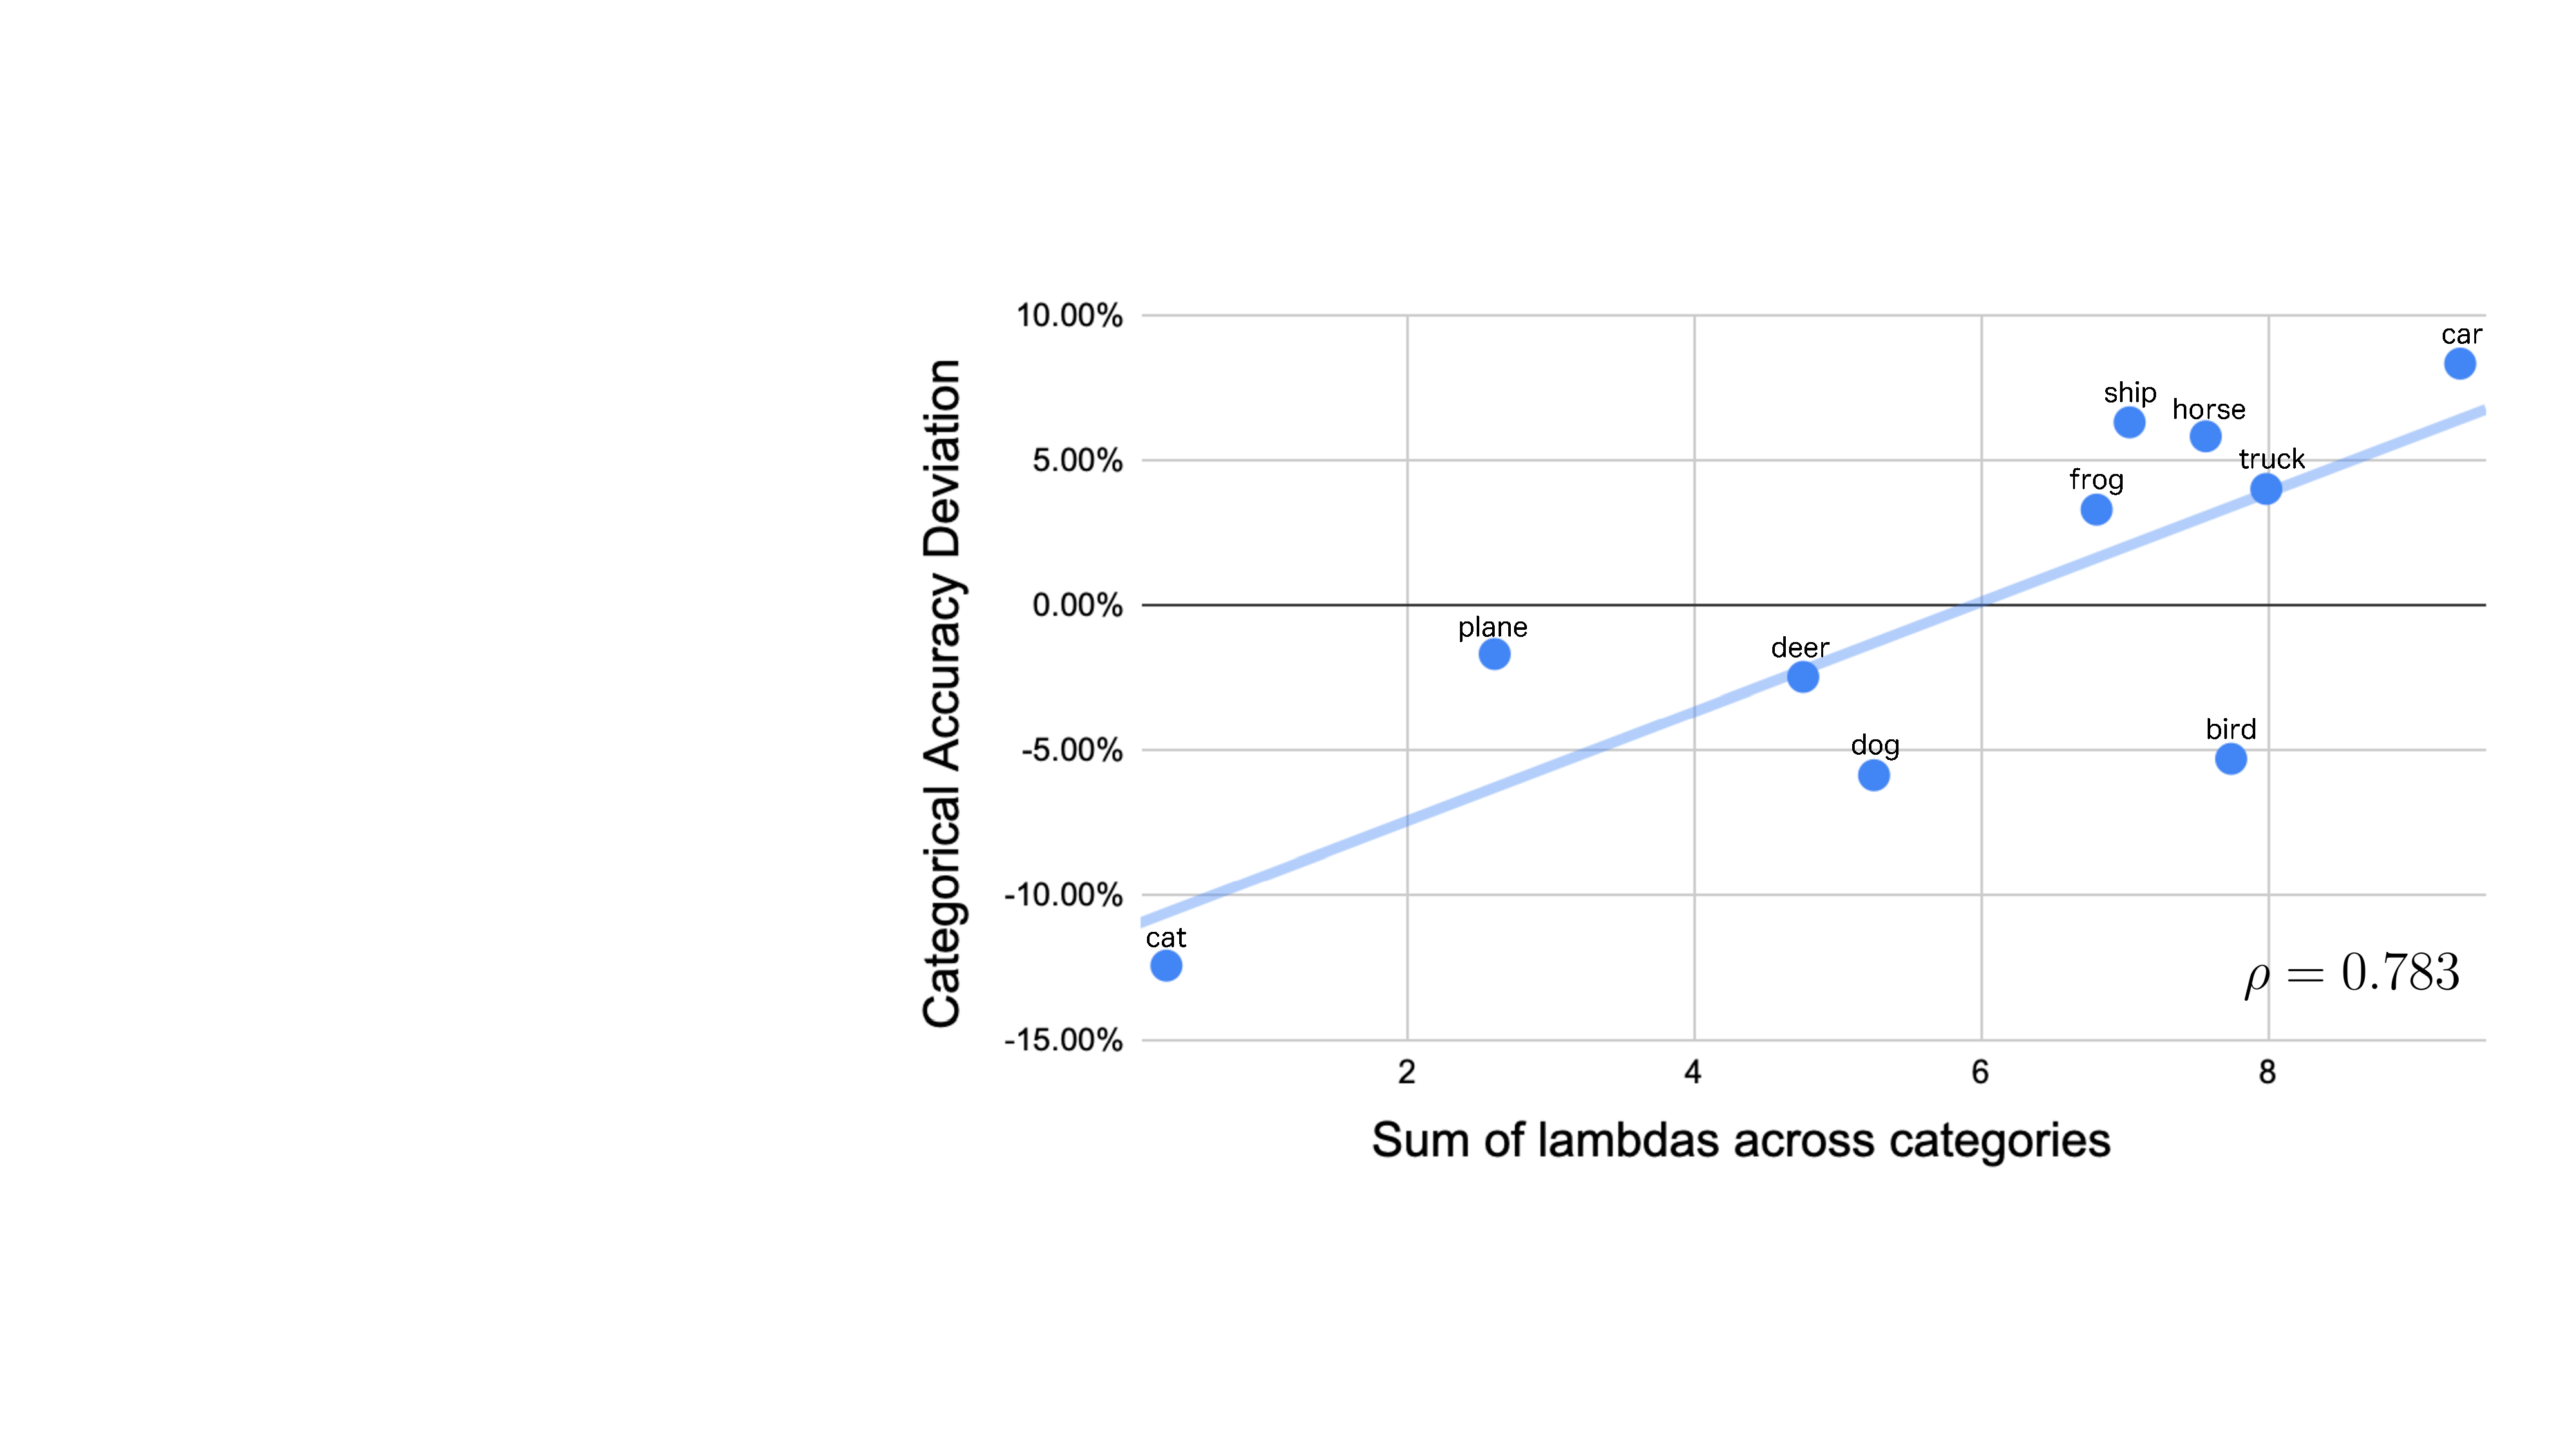
\includegraphics[width=\linewidth]{./figure/pearson.pdf}
%     \label{fig:correlation}
%   \end{subfigure}
%   \caption{Characteristics of DSVs; (Left) Entropy change of DSV candidates over time, (Right) Correlation between classwise mean test accuracy and the sum of $\lambda$'s}
%   \label{fig:DSV_characteristics}
% \end{figure}
\begin{figure}[t]  
  \centering
  \resizebox{0.8\linewidth}{!}{%
    \begin{subfigure}[b]{0.47\linewidth}
      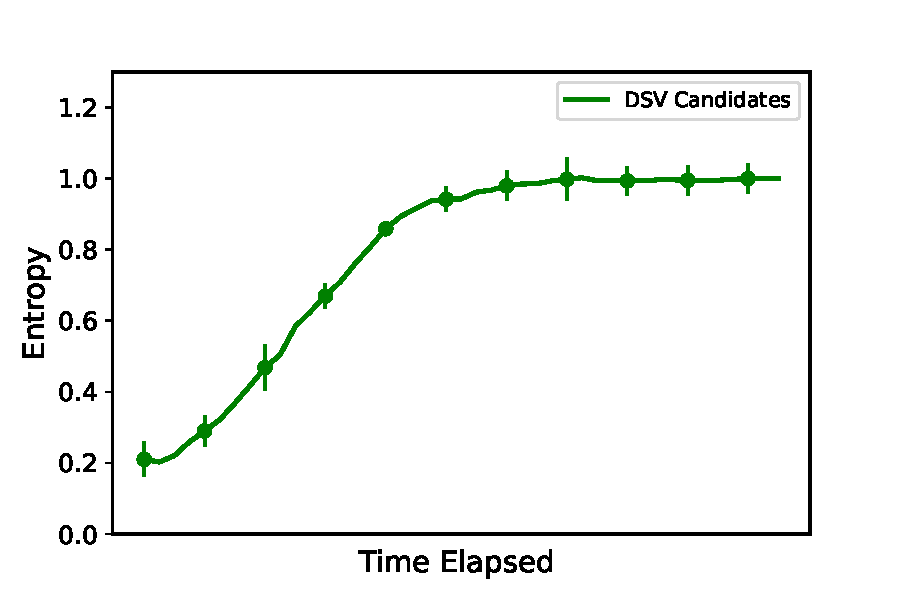
\includegraphics[width=\linewidth]{./figure/Entropy_DSV.pdf}
      \phantomcaption
      \label{fig:lambda_entropy}
    \end{subfigure}
    \hfill
    \begin{subfigure}[b]{0.53\linewidth}
      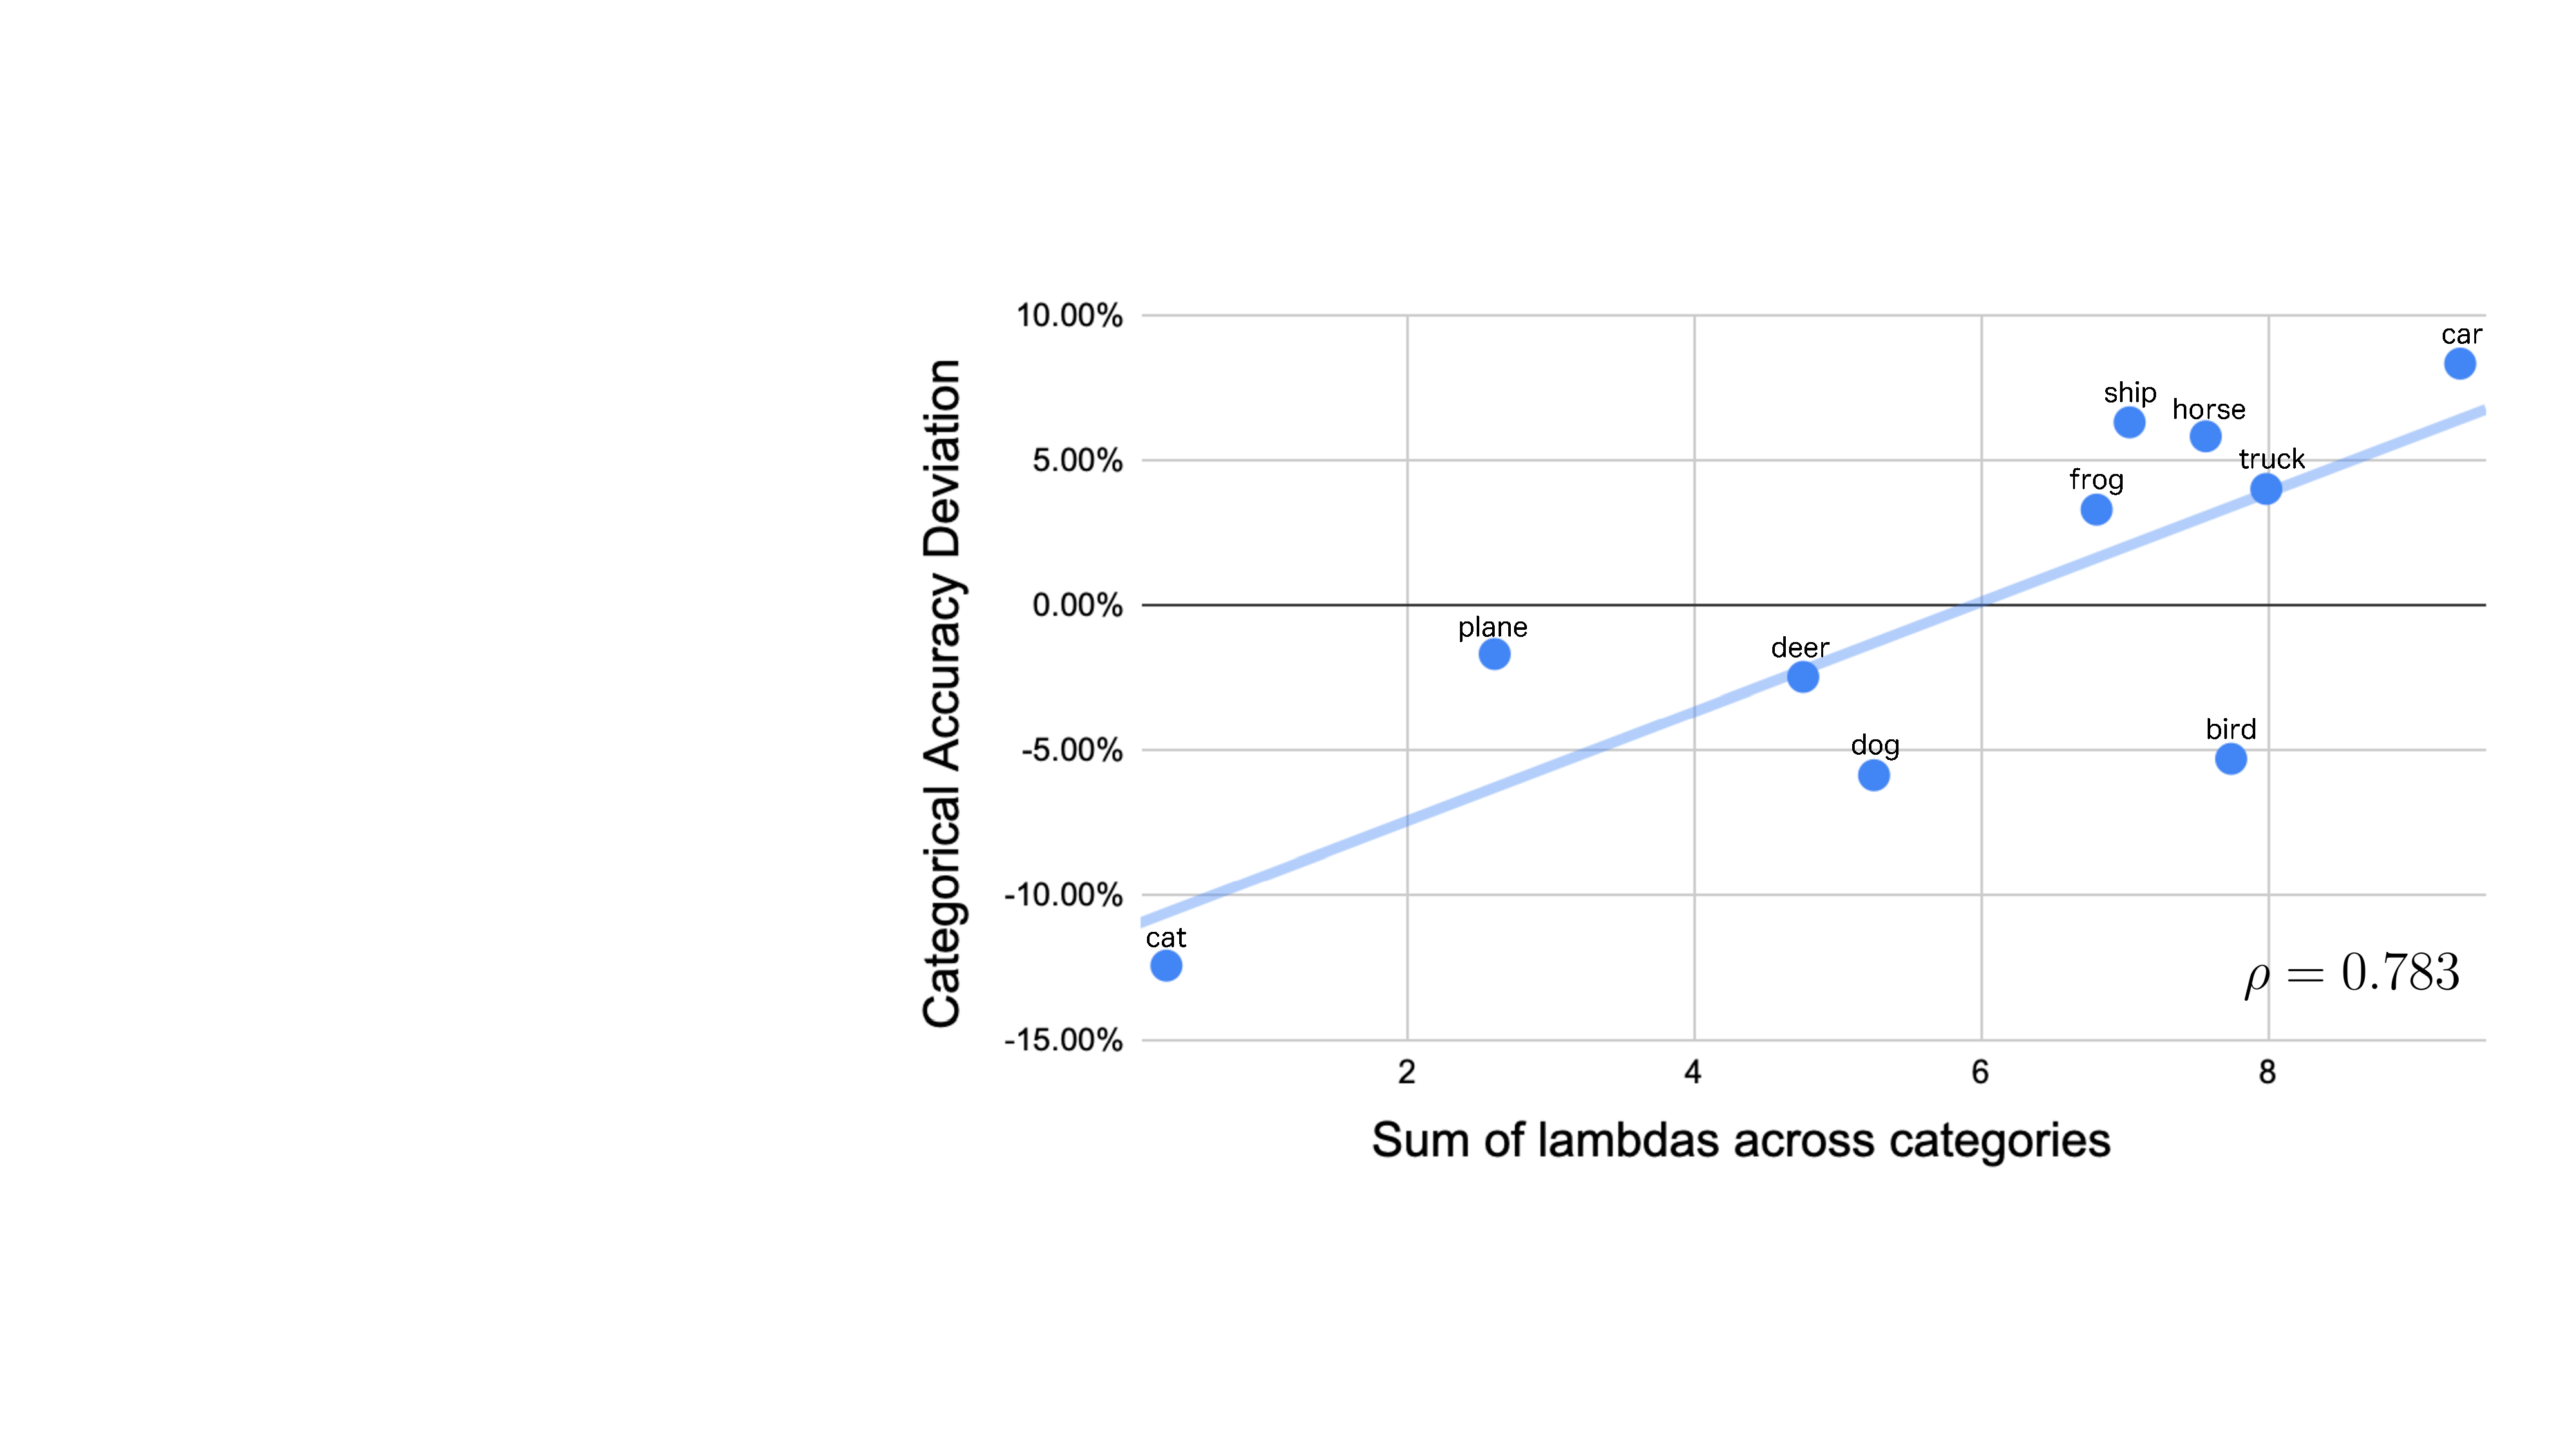
\includegraphics[width=\linewidth]{./figure/pearson.pdf}
      \phantomcaption
      \label{fig:correlation}
    \end{subfigure}
  }
  \caption{Characteristics of DSVs; (Left) Entropy change of DSV candidates over time, (Right) Correlation between classwise mean test accuracy and the sum of $\lambda$'s}
  \label{fig:DSV_characteristics}
\end{figure}


% \begin{figure}[t]  
%   \centering
%   \begin{subfigure}[b]{0.48\linewidth}
%     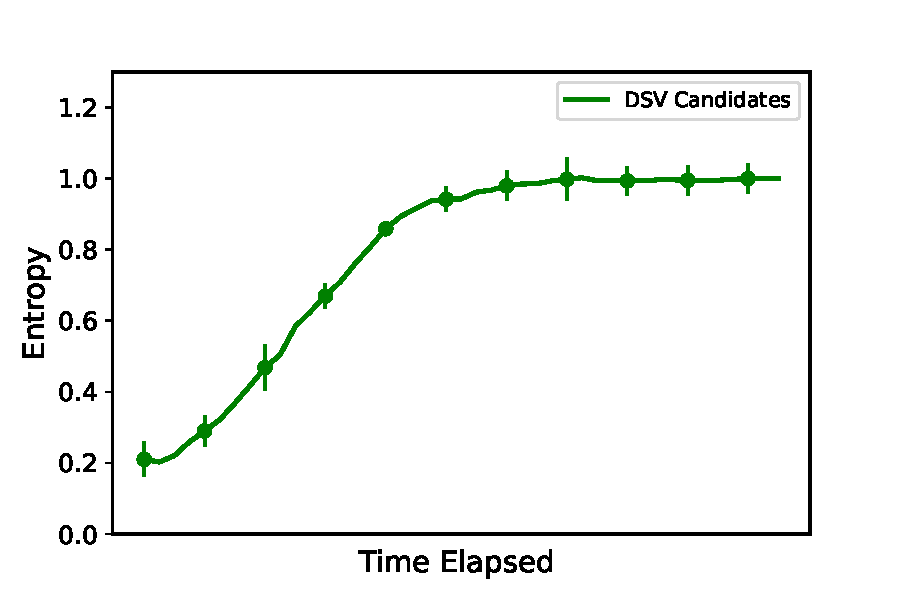
\includegraphics[width=\linewidth]{./figure/Entropy_DSV.pdf}
%     \label{fig:lambda_entropy}
%   \end{subfigure}
%   \hfill
%   \begin{subfigure}[b]{0.48\linewidth}
%     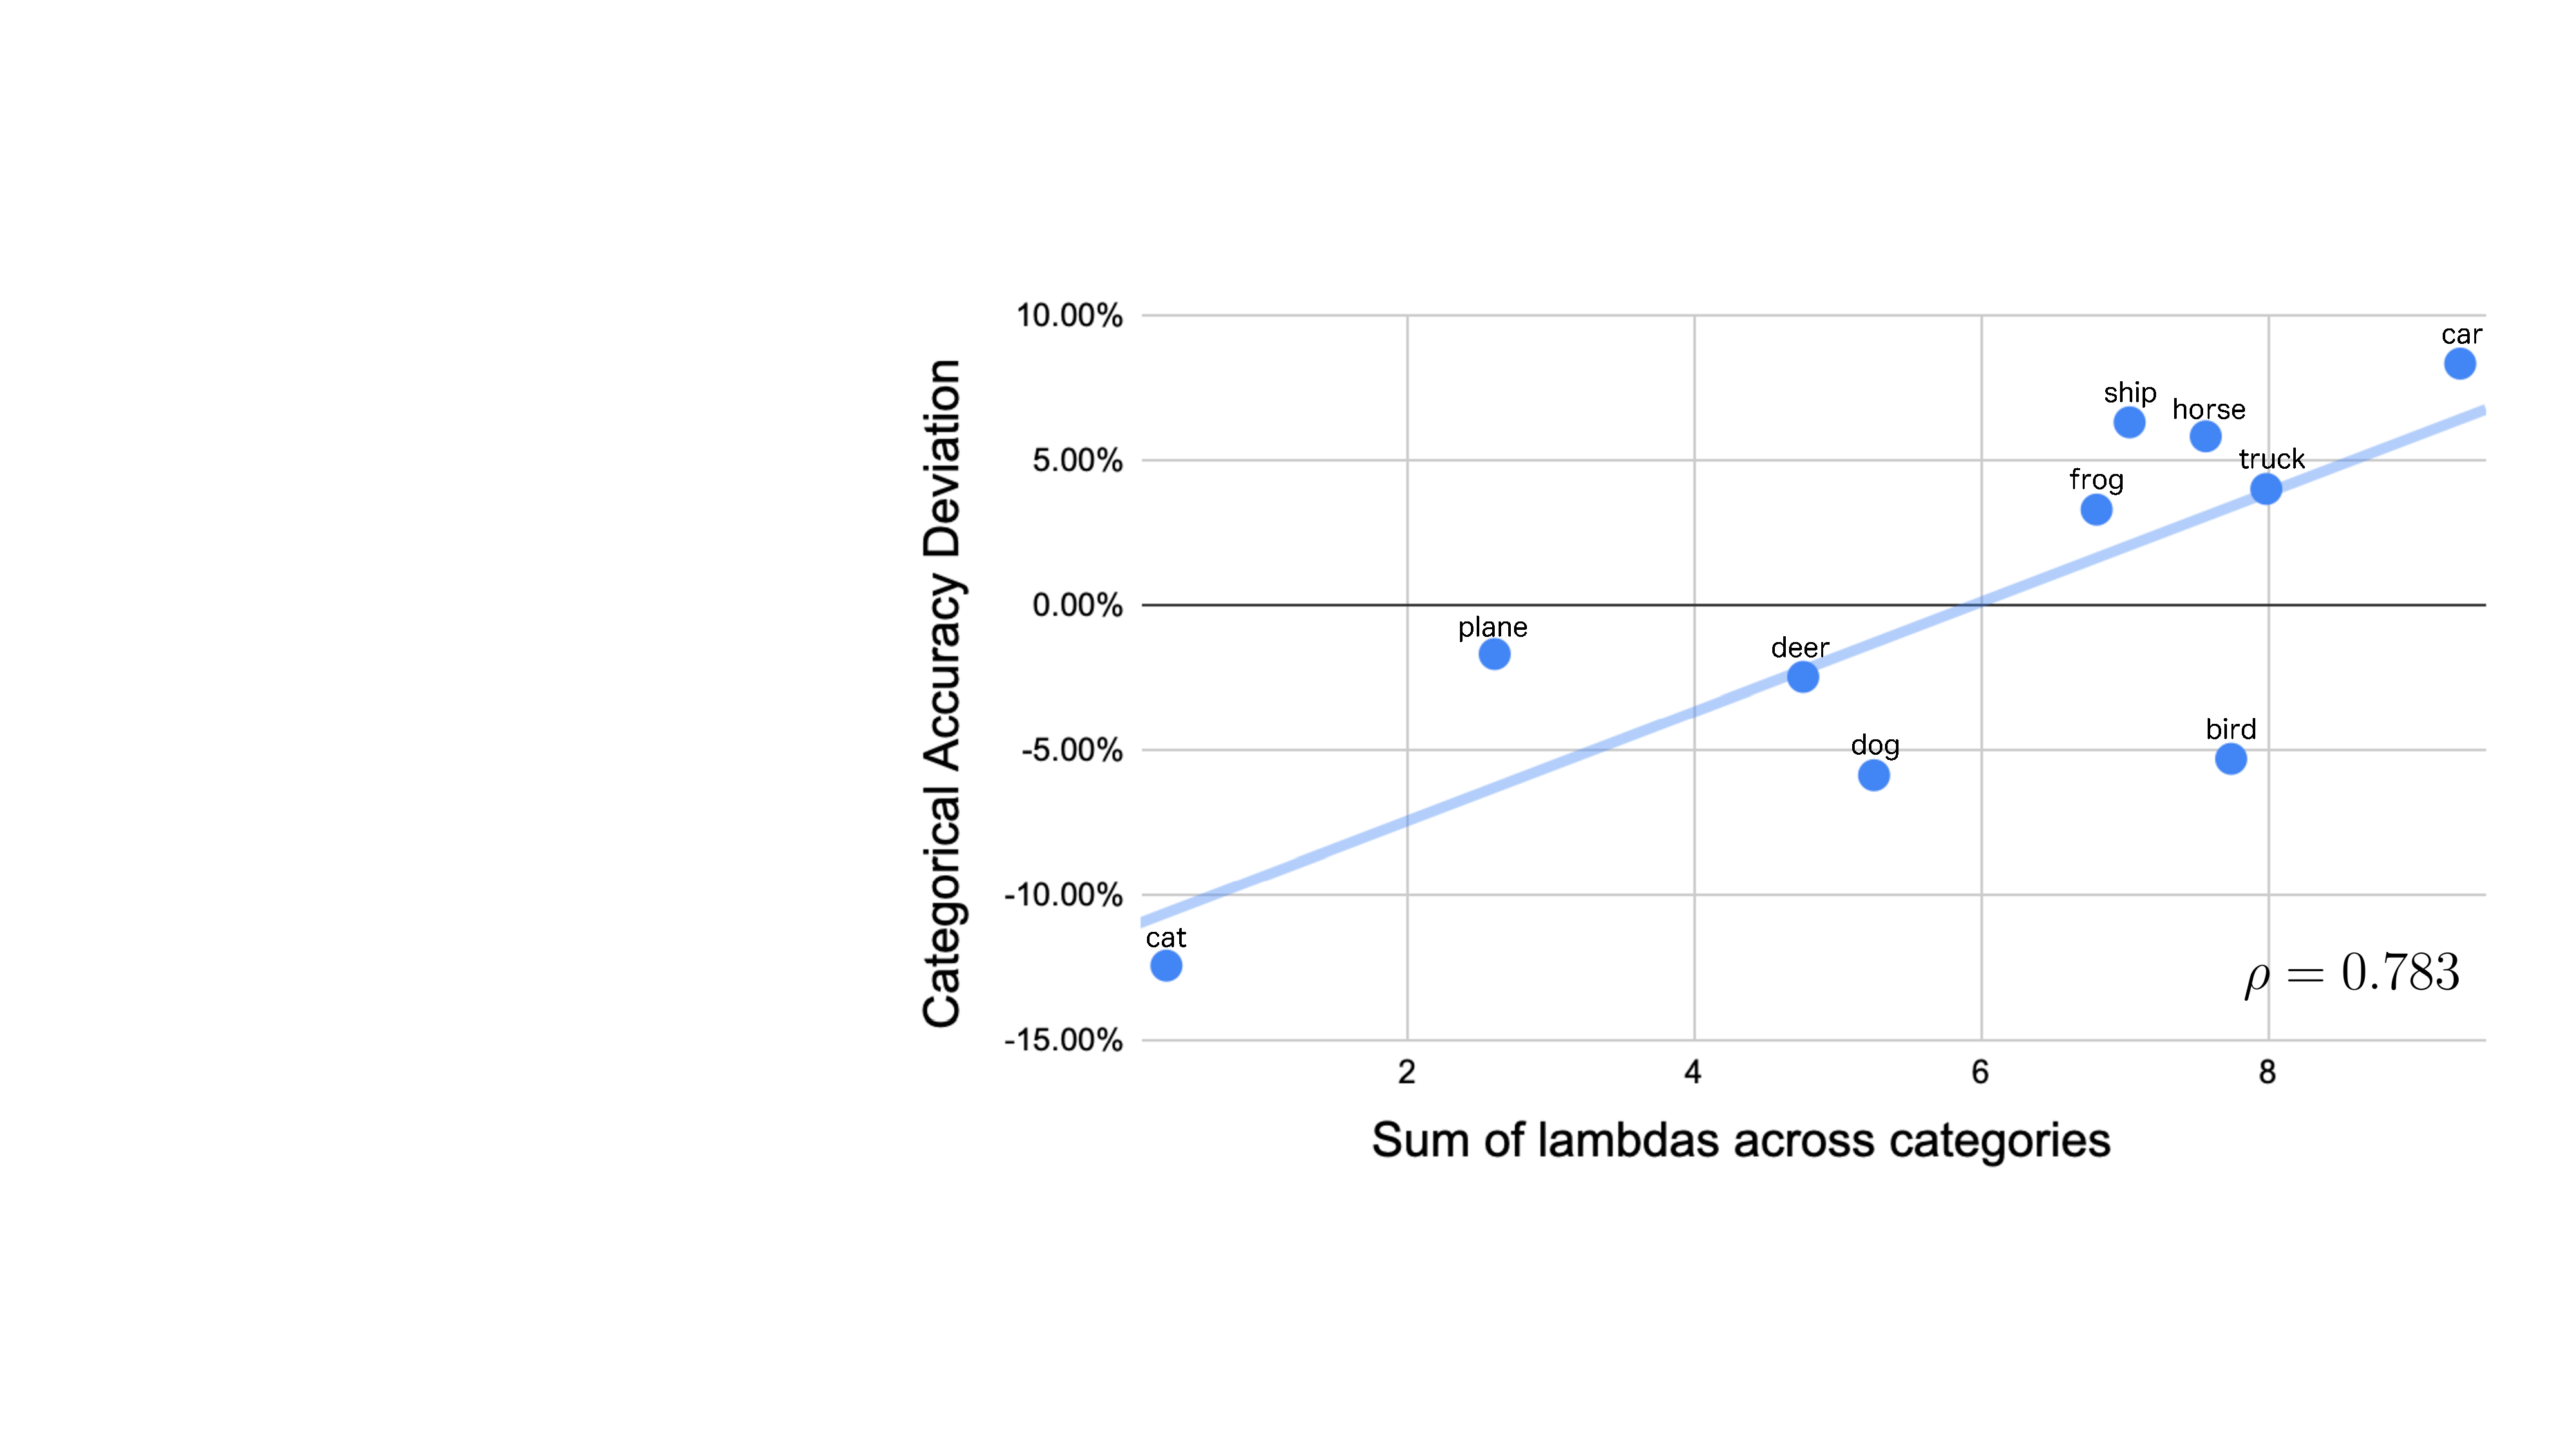
\includegraphics[width=\linewidth]{./figure/pearson.pdf}
%     \label{fig:correlation}
%   \end{subfigure}
%   \caption{\nj{Characteristics of DSVs}; (Left) Entropy change of DSV candidates over time, (Right) Correlation between classwise mean test accuracy and \nj{the} sum of $\lambda$'s}
%   \label{fig:DSV_characteristics} % 캡션 바로 다음에 라벨을 위치
% \end{figure}


Here, $L$ can be any loss function %with an exponential tail that is used in supervised learning, 
and we have employed the cross-entropy loss in our experiments.

\paragraph{Stationarity}
Secondly, the stationarity condition can be used directly as a loss function. Since we are extracting DSVs from the trained model $\Phi(\cdot ; \theta^*)$, %$\tmodel$, 
we construct this loss as follows:
%
\begin{equation}\label{eq:stationarity}
\hh{L_{\text{stat}} = D(\theta^*, -\sum_{i=1}^n \lambda_i \nabla_\theta L(\Phi(x_i;\theta^*), y_i))}.
\end{equation}
%
% \jh{이 섹션에서는 DSV가 만족해야하는 구체적인 조건을 제시하고, 그 조건을 만족하는 first-order computation cost의 optimization loss를 정의할 수 있음을 이야기한다.}
% \subsection{\jh{KKT condition in Deep Learning}}
%
% \jh{\ref{eq:DeepKKT}에서 우리는 deep learning에서의 KKT 조건에 대해서 알아보았고, 우리는 이 조건을 통해서 loss를 formulate 할 수 있다. 여기서 주의해야할 점은, 우리는 모델 $\Phi$를 만드는 것이 아닌 support vector를 만드는 것이다.}
%
% \paragraph{Primal feasibility}
% \jh{첫째로, primal condition은 기본적인 모델의 성능에 대해서 물어보는 조건이다. 즉 주어진 training data에 대해서, 모델은 training data를 제대로 판별할 수 있어야 하고, 특히 support vector도 마찬가지이다. 따라서, support vector는 첫째로 제대로 classify 되어야 한다.}
%
% \begin{equation}\label{eq:primal}
%     L_{\text{primal}} = L(\tmodel(x_s), y_s)
% \end{equation}
%
% 이때 $L$은 supervised learning에서 사용하는 임의의 expotentaial tail을 가진 함수를 사용하면 되고, 우리는 cross-entropy loss를 사용하였다.
%
% \paragraph{Stationarity}
% \jh{둘째로, 우리는 stationarity 조건을 직접적으로 loss로서 사용할 수 있다. 우리는 학습된 모델 $\tmodel$에서 DSV를 뽑아내는 조건이므로, 해당 loss는 다음과 같이 만든다}
%
% \begin{equation}\label{eq:stationarity}
%     L_{\text{Stat}} = D(\tmodel,  \sum_{i=1}^n \lambda_i {y_s}_i \nabla_{\theta} \Phi(\theta^*; {x_s}_i))
% \end{equation}
%
For the distance measure $D$, any metric can be used; we have chosen to use the $l_1$ distance to suppress the effect of outliers. It is crucial to remember that our objective is to find DSVs and the optimization is done for the primal and dual variables $x_i$ and $\lambda_i$ and not for the parameter $\theta$. %We have optimized only with respect to primal variable $x_i$ and the dual variable $\lambda_i$. 
For this, we require one forward pass and two backward passes; one for $\nabla_\theta L$ and the other for $\nabla_{x_i} D$. The overall computational cost is quite low, as we optimize only a small number of samples.

Moreover, as shown in \nj{Algorithm~\ref{alg:KKT} (Appendix \ref{sec:alg})}, 
we satisfy the dual condition by ensuring the Lagrange multipliers $\lambda_i$'s are greater than zero and disqualify any $x_i$'s from being a support vector candidate if during optimization $\lambda_i$ becomes less than zero. The condition that is not \nj{explicitly} satisfied is the complementary slackness. To directly fulfill the functional boundary for support vectors as specified in Sec.~\ref{sec:KKTcondition}, we would need to be able to calculate the distance between functions, which is not only abstract but also requires a second-order computation cost. Therefore, we adopted a relaxed version of the KKT conditions that excludes this requirement. Furthermore, as demonstrated in Sec.~\ref{sec:slackness}, we have shown that DSVs implicitly satisfy the complementary slackness condition. This implies that DSVs meet every condition introduced in conventional SVM.

% \jh{Furthermore, the stationarity condition reflects the dynamics of overparameterized deep learning models. We provide an analogy in Appendix~\ref{sec:overparam}.}



% \begin{figure}[t]
%   \centering
%    \includegraphics[width=0.9\linewidth]{./figure/redline.png}
%    \vspace{-5mm}
%    % \caption{Overall Idea of our algorithm. \hh{As primal and stationary conditions form a \nj{decision boundary which is a} subspace, we make use of an additional manifold (invariance) condition to meet our solution lies in \nj{the} data manifold. Initially sampled from noise, the DSVs gradually shift to become samples \nj{at the intersection the decision} boundary and the data manifold. %, achieved through only first-order computation. 
%    \caption{Conceptual overview of our algorithm. Initially sampled from noise, the DSVs evolve to intersect with the KKT solution subspace and the data manifold.%, achieved through only first-order computation. 
%    } 
%    \label{fig:manifold}
%    %\vspace{-2mm}
% \end{figure}




\paragraph{Manifold Condition: Reflecting High-Dimensional Dynamics of Deep Learning}

%In addition to satisfying the conventional KKT conditions, we have adopted additional criteria for determining DSVs. 
As modern deep learning deals with extremely high-dimensional spaces, imposing additional constraints other than the primal feasibility and stationarity conditions is needed so that DSVs reside in the desired data manifold. To achieve this, we add a manifold condition, which enforces that the DSVs lie on the data manifold. By selecting DSVs that are in the intersection of the solution subspace and the data manifold, we can properly represent both the model and the training dataset.

%As much as determining the data distribution in a high-dimensional space, giving additional constraints will allow DSVs to approach the desired data manifold. 
%\jh{As modern deep learning deals high extremly high-dimensional, the primary and stationarity and primary conditions does not construct exact solution, it constructs a subspace. Which implies 
%it does not guarantee that it is on the data manifold that the data is trained on. Among the DSVs that satisfy the \nj{Deep}KKT conditions, 
%we must select the `good' DSVs among the subspace. To do so, we add \textit{manifold} condition, which enforces the DSVs lie in data manifold.  By selecting DSVs that are in the intersection of the \nj{solution subspace} and the data manifold, it will be possible to properly represent both the model and the training dataset.}

To extract DSVs from the manifold, we assume that the model is well-trained, meaning it maintains consistent decisions despite data augmentation. In other words, the model should classify DSVs invariantly even after augmentation. To ensure this, we enforce that the augmented DSVs ($\mathcal{A}(x)$ \jh{where $\mathcal{A}$ denotes augmentation function}) also meet the primary and stationarity conditions.

%\jh{To extract DSVs from the manifold, we assume that the model is well-trained, Meaning the model does not change its decision among augmentation. %Inverting this idea, we propose that, when evaluating images within the manifold, an effective model should assess them in an augmentation-invariant fashion. 
%Put differently, the model should classify DSVs invariant even after augmentation. To do so, we enforce the augmented DSVs also meet primary and stationary condition.}
% Also, we exploit well-known image priors. We adop}
% Inverting this idea, we propose that, when evaluating images within the manifold, an effective model should assess them in an augmentation-invariant fashion. Put differently, the DSVs we identify should remain as DSVs even after augmentation. 

Also, we exploit traditional image prior \cite{total_prior, total_prior1}, total variance $L_\text{tot}$ and size of \nj{the} norm $L_{norm}$ \nj{to} make DSVs lie in \nj{the data} manifold. $L_\text{tot}$ is calculated by summing the differences in brightness between neighboring pixels, \nj{reducing} unnecessary noise in an image, and \nj{maintaining} a natural appearance. $L_{norm}$, \nj{taking a similar role,} penalizes the outlier and preserves important pixels.

\nj{Finally our DSV is obtained as follows where $\mathbb{E}_\mathcal{A}$ represents expectation over augmentations:}
\begin{equation} \label{eq:main_equation}
\text{DSV} = \argmin_x \mathbb{E}_\mathcal{A}  \left[L_{\text{stationarity}}(\mathcal{A}(x)) + \beta_1 L_{\text{primal}}(\mathcal{A}(x)) +  \beta_2 L_{\text{tot}}(x) + \beta_3 L_{\text{norm}}(x)\right].
\end{equation}

% \nj{적절한 manifold 상에 있다면 decision boundary가 sample들의 평균과 가까울 것이므로 probability를 높여준다고 볼 수 있다... 등으로 설명가능하지 않을까? 왜 decision boundary 근처의 sample들이 data를 대표하는지를 얘기할 때}

\nj{One might wonder if there is a better sampling strategy than using DSVs, such as sampling far from the decision boundary instead of near it. We argue that in a high-dimensional data manifold, most data points are located close to the decision boundary because, in a data-scarce, high-dimensional space, every sample matters and thus would serve as a DSV.}

%\nj{It is important to note that when sampling from a high-dimensional manifold, we are not merely selecting the nearest neighbors of the class means in a Euclidean parameter space. Instead, we are sampling from the manifold of the dataset as transformed by a well-trained deep model. This deep model reshapes the original data manifold into a well-defined form that generalizes effectively. Consequently, the data manifold is not a rough, non-separable space but rather a smooth, separable one. Thus, sampling from the decision boundary of this manifold involves: 1) Selecting images that satisfy the maximal margin criterion, and 2) Ensuring these images contain distinct, generalizable features for each class.}

%\jh{It \nj{is} important to note that when sampling from a high-dimensional manifold, we are not merely selecting the nearest neighbors \nj{of the class means} in a \nj{Euclidean parameter space}. Instead, we are sampling from the manifold of the dataset transformed by a well-trained deep model. The deep model reshapes the original data manifold into a well-defined form that generalizes well. From this perspective, the boundary of the dataset manifold is not a rough, non-separable space in the parameter space but rather a smooth, 
% one. Therefore, sampling from the boundary of this manifold means: 1) Sampling images that satisfy the maximal margin criterion. 2) Containing distinct, generalizable features for each class.}
% \jh{명심할 것은, 우리가 high-dimensional manifold에서 샘플링 할 때, its boundary에서 sampling한다는 것은 단순히 $l_2$와 같은 ㅔarameter space에서 class별로 neariest neighbor를 뽑는 게 아니라, \textbf{잘 학습된 deep learning model 상에서 변환된 dataset의} manifold라는 것이다. 딥러닝 모델은 기존의 data manifold를 변형시켜서, generalization이 잘 되는 well-defined 형태로 reshaping 하게 된다. 이 관점에서 dataset manifold의 boundary는 parameter space상에서의 separated 되지 않는, 그런 거친 공간이 아니라 매끈하고, separable한 공간이 된다. 따라서 이 manifold의 boundary에서 샘플링 한다는 것은 1. Maximal margin을 만족하는 2. 각 class별로 dintinct한, generalizable feature를 담고있는 image를 sample한다는 것을 의미한다.}


% \begin{equation}
    % DSV = \argmin{x}E_\
% \end{equation}


% \hh{In addition to satisfying the conventional KKT conditions, we have adopted additional criteria for determining DSVs. This idea stems from the unique challenges of deep learning in high-dimensional spaces, as opposed to traditional machine learning approaches, as can be inferred from \ref{fig:manifold}. We conduct optimization within the input dimension, which, as seen in the figure, forms a subspace of solutions. Among these, we must identify the 'good' DSVs, and to do so, we seek DSVs within the data manifold. Since the model is trained on the data manifold, it follows that the DSVs would also be formed within this manifold.}





% \paragraph{\jh{Connection to Diffusion models}}

% \jh{For DSV synthethis, we start DSV from noise, which is obtained from gaussian distribution. Can view this procedure as diffusion procedure.}

% \jh{A discritized diffusion model with classifier guidence follows following eqation.}
% \begin{equation}
% x_{t+1} = x_t + \epsilon_t \cdot \left( \nabla_x \log p(x_t) + \lambda \nabla_x \log p(y | x_t) \right)
% \end{equation}

% And this equation is similar to our algorithm~\ref{alg:KKT}, as our algorithm can be written as

% \begin{equation}
% x_{t+1} = x_t + \alpha \cdot \left( \nabla_x L_{\text{stat}}(x) + \lambda \nabla_x L_{\text{primal}} \right)
% \end{equation}

% Which means, stationaricy condition becomes `score` in terms of diffusion and primal condition can be viewed as `guidence`. This formulation makes sense as our procedure is similar to diffusion process. DSV starts from noise, \ie we sample its initialization from gaussian distribtuion. And our goal is to generate DSV throughout our algorithm. Which is in $\partial \mathcal{M}$. A boundary of manifold. Which means, DSV process moves gaussian contribution $\mathcal{N}$ to $\partial \mathcal{M}$
% we conducted experiments on classifier guidence in Sec.~\ref{sec:diffusion} 

%An assumption used by SSL is that a good model should be augmentation-invariant. 
%Inverting this idea, we posit that for images residing within the manifold, a good model should judge them in an augmentation-invariant manner. In other words, the DSVs we identify should remain as DSVs even after augmentation.

% This concept can also be interpreted from the perspective of Lie theory. When training models, we desire them to be \hh{semantic invariant} in any category, much like humans. That is, we hope the model yields the same result whether an image is shifted, slightly rotated, or flipped. While we may design models to inherently satisfy these properties, trained models also learn to treat images as Lie-equivalent. By requiring this \hh{semantic invariance} in the trained support vectors, we ensure that they satisfy the necessary condition of residing within the image manifold.

% \hh{relwork 위로 올리고, difference from previous work,,,}
% In fact, there was a paper that employed the KKT conditions as a loss similar to ours, focusing particularly on the stationarity condition. However, their objective was the opposite of ours. They viewed the KKT conditions merely as a prerequisite for model complexity and problem difficulty, suggesting that meeting these conditions alone does not guarantee that a vector will be a support vector. Our study, on the other hand, utilizes the KKT conditions more extensively. While the previous research did not employ the full spectrum of KKT conditions, we incorporated them broadly in our analysis. Their work initiated from the mean of the training dataset to address the data manifold problem, but our research begins with random noise. Additionally, they imposed the structure of SVMs onto conventional deep learning to address equivalence issues, mainly using full batch processing and focusing on binary classification problems. In contrast, our research adheres to the foundational deep learning settings of SGD, mini-batch, multi-class classification, and a limited number of support vectors. These distinctions highlight the unique contributions of our work compared to the previous study.

% \hh{이전 논문에 대한 얘기들은 찾아 보니깐 relwork에 다 있는것같아서 우리 논문의 차별점을 강조하는느낌으로 다시씀 }

% 이때 $D$는 임의의 distance measure면 되고, 우리는 $l_2$ distance를 사용하였다. 이때 명심해야할 것은, 우리가 구하는 것은 DSV라는 것이다. 우리는 $x_s, \lambda$에 대해서만 optimize하였다. 따라서 이 term을 계산할 때 first-order의 computation cost만 필요하다.

% 또한, algorithm \ref{alg:KKT}에서 보듯이, 우리는 dual condition를 lagrange multiplier $\lambda$ 자체를 0보다 크게 만들고, 그리고 optimize 과정에서 $\lambda$가 0보다 작아지는 $x_s$를 아예 support vector candidate에서 탈락시키는 것으로 만족하였다. 이중 우리가 직접적으로 만족시키지 않은 것은 Complementary slackness이다. 이는 우리가 support vector에 대해서 functional boundary \ref{sec:KKTcondition}을 직접적으로 만족하려면, 우리는 함수 사이의 거리공간에 대해서 구할 수 있어야 하는데 이는 abstract할 뿐더러 second-order computation cost를 요구하기 때문에 해당 조건을 제외한 relaxed KKT condition을 만족하도록 하였다.

% \begin{algorithm*}\label{alg:KKT}
% \caption{Support Vector Refinement for Deep Learning Model}
% \begin{algorithmic}[1]
% \Require Trained model $\tmodel$augmentation functor $A$
% \State Initialize $\mathbf{x_s}$ with random noise, \text{Num\_Class}, \ast\text{image\_shape})$
% \State Initialize $\mathbf{y}$ with shape $(\text{Num\_Samples}, \text{Num\_Class})$
% \While{not converged}
%     \State Compute primal loss $L_{\text{primal}} = L(\tmodel(x_s), y_s)$
%     \State Compute stationarity loss $L_{\text{Stat}} = D(\tmodel,  \sum_{i=1}^n \lambda_i {y_s}_i \nabla_{\theta} \Phi(\theta^*; {x_s}_i))$
%     \State Update $\mathbf{x}$ and $\lambda$ to minimize $L_{\text{primal}}$ and $L_{\text{Stat}}$
%     \State Evaluate dual condition, remove support vector candidates where $\lambda<0$.
% \EndWhile
% \end{algorithmic}
% \end{algorithm}


% \hh{ Linearly seperable dataset과 monotone, decreasing, differentiable loss function에 대하여 gradient decent로 구한 W(t)(의 크기는)는 무한대로 발산한다. Regularized W(t)의 극한은 hard margin solution SVM인 $\hat{w}(t)$의 regularized term으로 수렴하는데, $\hat{w}(t)$는 support vector들의 합으로 표현할 수 있다. 이때의 $\nabla L $은 exponential tail의 영향으로 dominant한 몇개의 support vector들의 합으로 근사될 수 있으며, 따라서 KKT stationary  condition을 활용하여 $\Delta_{\text{KKT}}$ =  $|\mathbf{W}_f - \Sigma^i \lambda_i\nabla L(\mathbf{x_i}, \mathbf{y})|$ 로 kkt loss를 구성할 수 있다. 따라서 충분히 기학습된 W와 주어진 L에 대하여 $x_i$에 대한 gradient update를 통해서 support vector들을 구할 수 있다.  
% 결국 KKT condition을 어떻게 활용하여 suppport vector을 구할것이며, 이 방식의 정당성에 대해서 설명할 필요가 있어서 이런 내용을 어딘가 넣는게 좋을것 같은데 어떻게 생각함?}

% 결국 이것이 원하는 것은, binary classification에서 model이 input x를 명확히 구분하는 것 뿐만 아니라, 그 margin을 1 밖으로 밀어내는 것을 뜻하는 것이다. 이는 $sign(f(x)) = y$임을 의미하고, 다시 말해서 이는 모델이 x를 정확하게 classify 했다는 것을 의미한다.

% 따라서 우리는 해당 조건을 만족하는 x와 lambda들은 relaxed KKT condition을 만족한다는 것을 알 수 있는데, 우리는 해당 조건을 만족하기 위햐여 다음과 같은 전략을 사용한다.

% 여기서 직접적으로 적용하기 어려운 부분은, margin의 크기를 exact하게 1로 맞추는 과정이다. margin의 크기를 1로 맞춘다는 것은 거리를 사용한다는 것을 의미하고, abstract한 parameter manifold상에서의 거리를 잰다는 것은 metric tensor가 필요하다는 것을 의미한다. 하지만 metric tensor의 크기는 number of parameter의 square이고, 이는 Hessian의 computation cost와 같다. 따라서 first-order 알고리즘만 사용하는 일반적인 딥러닝 알고리즘에서는 사용되기가 매우 어렵다. 따라서 우리는 relaxed된 KKT condition을 사용하는데,
% \hh{relaxed KKT condition이 뭔지에 대해서 간단하게 알려주면 좋을듯?? 사실 나도 이게 뭔지 정확히 몰라서..}

% $L_stat, L_primal$ 위 두개를 사용하고, 매 training epoch마다 lambda가 0보다 큰 아이들만 고르게 되면, 모든 조건을 만족한다고 생각할 수 있다. 따라서 우리가 가하는 조건은 KKT condition에서 metric에 대한 고려만을 제외한 가정이라고 할 수 있다.


% 이거 말고 다른 적합한 말로 하자.

% 하지만 우리가 위 조건만으로 다 한다고 볼 수는 없는데, 왜냐하면 저 조건을 만족하는 x는 충분조건이 아니라 필요조건이기 때문이다. 우리가 x에서 w를 구할때, 우리는 $x\in \mathcal{D}$ 에서 $w$를 구한다. 하지만 만약 반대로 $w$ 에서 $x$를 구하게 되면, 우리는 그 조건을 무시한다. 만약 차원이 낮다면, 그것은 큰 문제가 되지 않는다. 왜냐하면 manifold의 크기 자체가 이미지의 dimension과 큰 차이가 나지 않기 때문에 x가 data manifold 안에 있어야 한다는 조건은 따로 주지 않아도 되기 때문이다. 하지만 딥러닝의 경우는 machine learning과 다르게 high dimensional data를 다루고, 따라서 우리가 구한 해가 manifold 안에 있을 확률이 매우 낮다. 따라서 우리는 추가적인 조건을 통해서 x가 manifold 안에 있도록 해야 한다.

% 우리는 DSV를 구하기 위해, 기존의 KKT 조건을 만족하는것 외에 추가적인 조건을 차용하였다. 그 아이디어는 \ref{fig:manifold}에서 얻을 수 있는데, 왜냐하면 딥러닝이 기존의 머신러닝과 다르게 high-dimension에서 문제를 풀기 때문이다. 우리는 input dimension에서 optimization을 진행한다. 따라서 figure에서도 볼 수 있듯이, 그것을 만족하는 것들은 subspace를 형성한다. 우리는 이중 '좋은' DSV를 찾아야 하고, 이를 위해서 우리는 DSV를 data manifold 안에서 찾는다 model은 data manifold에서 학습하였기 때문에, 마찬가지로 DSV도 data manifold에서 형성될 것이기 때문이다.

% 우리는 DSV를 manifold에서 얻게 하기 위해 SSL의 철학을 차용한다. SSL이 사용한 assumption은 좋은 모델은 augmentation-invariant하다는 것이었는데, 우리의 아이디어는, 반대로 manifold 안에 있는 이미지를 좋은 모델이 판별할 때에, 그 모델은 augmentation-invariant하게 판단하여야 한다는 것이다. 다시 말해서, 우리가 구한 DSV는, augement 하더라도 여전히 DSV여야 한다는 것이다.

% 해당 아이디어는 lie thoery 측면에서도 해석할 수 있다. 우리는 모델을 학습할 때 있어서, 인간처럼 모델이 어떤 종류이든 abstract한 manner에서의 symmetric하기를 원한다. 다시 말해서, 우리는 image가 shift하더라도, 조금 rotate하더라도, flip 하더라도 모델이 같은 결과를 내기를 바라며, 우리는 모델이 이러한 성질을 자체적으로 만족하게 설계하기도 하지만 그것과 별개로 학습된 모델은 image들을 lie-equivalent하게 학습하기도 한다. 우리는 이러한 symmetry를 학습된 support vector에 요구함으로서, 우리는 support vector가 image manifold 안에 있어야 하는 필요조건을 만족하게 한다.

% 두번째 viewpoint는 self-supervised learning이다. 우리가 요구한 것은 augmented support vector가 여전히 support vector의 property를 만족하도록 하는 것이었다. 이는 정확히 SSL이 철학을 역순으로 접근한 것이다. SSL에서 원하는 것은 모델이 주어진 data distribution에 대해서 augmentation-invariant하도록 학습하는 것이다. 그리고 우리가 요구한 것은 우리가 학습하고자 하는 데이터가 pretrained model에 feedforward 시켰을 때 augmentation-invariant하도록 하는 것이다. 따라서 이둘의 철학은 제대로 학습된 모델/데이터는 augmentation이 있더라도 그 정보량이 바뀌지 않아야 한다는 공통된 기반을 가지고 있다.

% \jh{사실, 이전에 우리와 비슷하게 KKT 조건을 사용한 페이퍼가 있었고, 이중 cite가 KKT condition의 stationarity condition을 사용하였다. 여기서 우리의 contribution recap. 우리의 loss 중작년 첫 페이퍼 중에 이런 페이퍼가 있었지만, (그러니까 stationarity condition)을 사용한 페이퍼가 있었지만, 이들의 목표는 model로부터 ~ 이들과 다른 점은, 우리의 목표와 그들의 목표는 정반대라는 것. 우리는 KKT condition을 필요조건으로서 보았으며, 모델이 복잡해지고, 풀고자 하는 문제가 어려워질 경우에 KKT condition을 만족하는 것 만으로 그것이 support vector가 될 확률이 if and only if라고 할 수 없다. 또한, 그들의 경우 KKT condition을 다 쓴거도 아니고, 우리가 KKT condition을 더 많이 활용하였으며, 이들은 그 manifold 문제를 풀기 위해서 initialization을 구하고자 하는 training dataset의 mean에서 시작하였다. 다시 말해서, 그들의 initialization point는 manifold 위였다. 그것에 반해, ours는 random noise에서 시작한다. 그것을 넘어서, 그들이 푼 문제는 SVM과의 등가성을 위해서 SVM의 구조를 conventional deep learning에 강요하였다. 먼저 full batch를 사용하였으며, binary classification 문제를 풀었고, support vector라는 말을 사용하지 않았고 그들은 KKT condition을 만족해야 하는 image를 클래스당 수천개로 잡아 그 위에서 학습하였다. 반면에 우리는 기본적으로 deep learning이 사용하는 세팅, SGD, minibatch, multi-class-classification, limited number of support vector를 사용하였다는 차이점도 더 있다.}

% \begin{enumerate}
%     \item overparmeterized condition, i.e., $n \leq d$
%     \item $L$ has expotential tail
%     \item A model is overfitted. i.e., model은 infintely-many epochs를 거쳤다 (\hh{얼마나 overfitted 되었을때인지를 명시하는게 어떨까. infinately  many epoch동안 학습시킨것에 대한 가정이 hold하기위한 real world(실험 환경) 조건에 대하여 명시하는게 어떨까. "seperable data" 논문에서도 logistic, CE loss converge  속도하고 gradient decent로 인해서 W가 converge 하는 속도가 다르기때문에 loss가 매우 작아도 W가 수렴할때까지 계속 학습시켜야한다고 했는데 ,실제 실험에서 이런 가정들을 만족하기 위해서 어떤 기준으로 converge threshold를 잡았는지 뒤에 실험이나 가정부분이나 넣어주는게 좋을것같아})
%     \item 이 경우에, $(X,Y) \in \mathcal{D_{\text{training}}}$ 을 넣는다면, $f(X) = Y$ 이다.
%     \item 또한, $f(\tilde{X}) = f(X)$ 이며, 이때 $\tilde{X}$는 X에 대해서 group action을 취한 것이다. (augmentateion)
% \end{enumerate}
% \hh{가정들이 왜 필요하고, 어디에 쓰이는지 명시하면 좋을듯? 1번 overparameterized condition -$>$dataset에 대한 solution이 무조건 존재해야 하므로(?), 2번+3+4번 조건 -$>$ weight의 residual converges(relative to the size of the weight) to zero so the weight/norm(weight) converges after infinite iteration
%  근데 4번 조건이랑 dataset is linearly seperable이 동치인가?}
% In this section, we talk about the existence of DSV and how to obtain it.

% \subsection*{Existence of Deep Support Vector}

% Proof sketch

% 1. 기본적인 틀은 그 이전에 있던 페이퍼에서 가져옴

% 2. 그니까 왜 support vector를 가지는지 이거는 걍 가져와서 설명하면 됨
% 이 다음, dataset reconstruction에서 SVM 조건과 같아지는 것을 보여주고, 
% 필요조건 하나를 내세움

% % 밑에 나올 내용은 KKT condition. 즉 | w - \sum_i\lambda_i\nabla{L(x_i)} | = 0  여야 한다는 것
% \begin{equation}
%     | w - \sum_i\lambda_i\nabla{L(x_i)} | = 0
% \end{equation}

% 이것에 대한 intuitive한 설명, 그러니까 gradient가 converge하면\dots

% 하지만, 이러한 가정은, $x_i$가 data manifold에 존재한다는 것을 가정하고 있다. 하지만 우리는 
% support vector를 data manifold 내에서 찾는 것이 아니라, parameter space에서 찾는 것이 목적이기 때문에,
